\documentclass{article}
\PassOptionsToPackage{numbers,sort&compress}{natbib}
\usepackage[preprint]{neurips_2026}
\usepackage[utf8]{inputenc}
\usepackage[T1]{fontenc}
\usepackage{amsmath,amsfonts,booktabs,graphicx,array}
\newcolumntype{L}[1]{>{\raggedright\arraybackslash}p{#1}}
\usepackage{microtype}
\usepackage{placeins}
\usepackage{pdfpages}
\usepackage[hidelinks]{hyperref}
\usepackage{url}
\urlstyle{same}
\hypersetup{pdftitle={Maintaining ECG Classification under Missing Leads with Supervised Lead Masking},pdfauthor={Wang Youyang},pdfsubject={MD6329 course project report}}
\emergencystretch=2em
\title{Maintaining ECG Classification under Missing Leads\\with Supervised Lead Masking}
\author{Wang Youyang\\Student ID: G2606821F\\Nanyang Technological University\\MD6329: Deep Learning for Healthcare}
\begin{document}

\includepdf[pages=1,pagecommand={\thispagestyle{empty}}]{cover_page.pdf}
\setcounter{page}{1}
\maketitle
\begin{abstract}
A remote ECG interpretation service may receive 12-lead, 6-lead and 2-lead recordings, and a classifier trained only on complete leads degrades when it receives a subset. We evaluate supervised random whole-lead masking, an existing intervention, under matched conditions. On PTB-XL version 1.0.3, model A is trained on complete inputs and model B on a 50/50 mixture of complete and randomly masked inputs, with the same network, patient-separated splits, training budget and checkpoint rule, and three paired seeds are evaluated on five diagnostic superclasses. On 2,158 held-out recordings from 1,877 patients, mean macro-AUROC over four reduced-lead configurations rises from 0.6908 to 0.8882, a prespecified paired gain of +0.1974 (95\% patient-bootstrap interval [0.1882, 0.2067]); under complete-input-only selection the arms differ by +0.001 [$-$0.001, 0.003] on complete input. Exploratory analyses compare this gain with stronger baselines. A two-step test-time repair of zero-filled A (deriving missing limb leads from the available ones, then re-estimating BatchNorm statistics) recovers most of the gap: B leads by +0.017 to +0.030 on the four configurations with similar calibration, and models trained for each configuration exceed B by about 0.02. Across 207 lead subsets, the repair matches B when at least two limb leads remain (+0.002), and B leads by +0.071 with fewer than two limb leads and by +0.110 with a single lead. A time-cutout control removing the same amount of information gains nothing. Masked training transfers to a limb-only lead family withheld from training, provided unavailable leads are detected and zeroed. Its value is one fixed model for any lead combination, clearly ahead of test-time repair when fewer than two limb leads remain; for a fixed, known configuration, a dedicated model performs best.
\end{abstract}
% Section body, v9.5 (2026-10-25): synced from report/full_report_v9_zh.md v9.5.
% Exploratory analyses are numbered E1--E13 (the unrun availability-indicator analysis has no number).
% This file is edited directly; the v8 generators (build_draft.py, assemble_paper.py) would overwrite it.
% Course citations give PDF pages and clickable video timestamps.

\section{Problem Formulation}

\subsection{Healthcare problem and research question}

Consider a remote ECG interpretation service that receives three kinds of recording: standard 12-lead ECGs from hospitals, two-lead recordings from ambulatory monitoring, and six-lead ECGs from handheld devices. Handheld devices are increasingly used by both healthcare workers and patients \citep{azram2021evalecg}; they have only three electrodes, two held in the hands and one placed on the left leg \citep{azram2021evalecg}, so they measure two independent voltages from which all six limb leads are computed \citep{reyna2022issues}. An ECG lead is one voltage signal measured between electrodes, and the standard 12 leads are obtained from ten electrodes \citep{presacan2025reconstruction}. If the service's automated classifier was trained only on complete 12-lead ECGs, it may quietly degrade on recordings with fewer leads, and the service has no way to report how reliable each output is for that lead configuration. Fewer leads carry less information: EVALECG Cardio found that a six-lead handheld device agreed well with the 12-lead ECG for rhythm assessment and less well for ischaemia and left ventricular hypertrophy \citep{azram2021evalecg}. In the 2021 PhysioNet challenge, most algorithms changed their average score by less than 2\% between twelve-lead and two-lead test data \citep{reyna2022issues}; the organizers note that this may not hold for subtler ST changes, and the diagnoses studied here, myocardial infarction, ST/T change and hypertrophy, depend on such morphological changes.

Existing work follows three routes: training or fine-tuning a separate model for each lead combination, as Oh et al.\ fine-tune one pretrained model per configuration \citep{oh2022leadagnostic}; reconstructing the missing leads before classification \citep{lence2025ecgrecover}; and letting a single model handle the different inputs directly \citep{fast2026af,liu2025kmerl}. The first route suits settings where the device type is known; missingness that is not known in advance, such as an electrode detaching during monitoring, calls for a model that handles any combination. The 12 leads admit 4,094 subsets \citep{zhang2026subsetbenchmark}. Even after accounting for limb-lead redundancy, 510 subsets remain informationally distinct: the limb leads have eight information states (none, one of six single-lead directions, or two or more, which determine all six), multiplied by the $2^6$ precordial combinations and minus the empty and complete sets, assuming the limb-lead relations hold exactly. Training a model for each is impractical. We take the third route, with the aim of reducing the avoidable loss of discrimination while keeping a single classifier and one output vocabulary.

Our primary research question is: \textbf{Does training one ECG classifier with both complete and randomly lead-masked inputs improve discrimination under predefined lead-unavailability conditions, compared with matched complete-input training?} Macro-AUROC is the mean of the five diagnostic labels' AUROCs; it measures how well the model ranks positive records above negative ones, is independent of any decision threshold, and equals 0.5 for random guessing. We hypothesized that, averaged over the four reduced-lead configurations, the masked-training model's macro-AUROC exceeds the complete-input model's; the decision rule is that the lower end of the primary effect's 95\% patient-bootstrap interval lies above zero. This rule and the six checkpoint hashes were fixed before the test labels were parsed (the study was not publicly pre-registered). Control arm A fills missing leads with zeros, which represents naive deployment; stronger baselines are tested in the exploratory analyses. Complete-input performance is reported as a descriptive endpoint, without a prespecified acceptable-loss margin. The primary result showed that the complete-input model deteriorates far more than the loss of information can explain, which led to a secondary research question formulated after the test: \textbf{Why does complete-input training fail, how much can be recovered without retraining, and where does masked training stand relative to the strongest training-free repair and to models trained for each configuration?} Further follow-ups ask whether the benefit extends to a lead family withheld from training, whether probabilities and fixed thresholds remain usable when leads are missing, and how the results depend on the representation of missing leads. All follow-up analyses were designed after the primary test and reuse the same test set, so they are exploratory.

The standard 12 leads form two groups. The six limb leads (I, II, III, aVR, aVL, aVF) are derived from the limb electrodes, and only two of them are independent: any two limb leads (for example I and II) determine the other four as exact linear combinations \citep{reyna2022issues}. On 2,000 PTB-XL training records, the median relative residual of these relations is about 0.5\%, and it is at most 1.2\% for 95\% of records. The other six, the precordial leads V1--V6, are placed on the chest. We adopt the four reduced-lead configurations of the 2021 PhysioNet challenge \citep{reyna2022issues}. S6 contains all limb leads, which corresponds to placing only the limb electrodes. S4 (I, II, III, V2) and S3 (I, II, V2) add one precordial lead, V2. S2 (I, II) is the configuration the challenge chose for the two-lead case, as the most common configuration in ambulatory monitoring \citep{reyna2022issues}. Because of the linear relations among the limb leads, S6 and S2, and likewise S4 and S3, carry approximately equivalent information, which later lets us test whether a model uses this redundancy. We study the problem on PTB-XL for five diagnostic superclasses, namely normal (NORM), myocardial infarction (MI), ST/T change (STTC), conduction disturbance (CD) and hypertrophy (HYP, covering both ventricular hypertrophy and atrial enlargement), under complete 12-lead input (S12) and the four configurations above. These superclasses form the top level of the PTB-XL diagnostic hierarchy and are a standard task in its benchmark \citep{strodthoff2021benchmark}. Compared with finer diagnostic statements, they have enough positive test records for stable AUROC estimates in every configuration; even HYP, the rarest, has 262. All configurations use the same compact residual CNN and preprocessing, with a matched complete-input-trained model as the baseline. We simulate lead unavailability by zeroing leads in PTB-XL's hospital 12-lead recordings.

The key techniques on all three routes have prior art, and we use a conventional residual CNN. The paper makes three contributions.
\begin{itemize}
\item \textbf{A prespecified matched comparison.} We evaluate supervised lead masking with identical architecture, initialization, record order, optimizer, training budget and checkpoint-selection rule, and report patient-level intervals conditional on three training seeds together with seed-level intervals. E1 examines how the shared selection rule affects the two arms differently.
\item \textbf{A repair ladder} (exploratory, designed after the test and reusing the same test set, as are all analyses below). Zero-filling creates inconsistent inputs and shifted activation statistics, and the two overlap. On the four protocol configurations, deriving the missing limb leads and re-estimating BatchNorm statistics closes 85\%--92\% of the gap (depending on the selection rule); masked training keeps an advantage of +0.017 to +0.030 and is about 0.02 below models trained for each configuration. Across 207 lead subsets, this repair matches masked training whenever at least two limb leads remain, and masked training's clear advantage appears on inputs with fewer than two limb leads. A time-cutout control that removes the same amount of information gains nothing.
\item \textbf{The scope of the result}: a limb-only lead family withheld from training, calibration at fixed thresholds, the representation of missing leads, and the agreement of MI-subclass performance with the anatomical coverage of the leads.
\end{itemize}
The prediction target is discrimination of ECG annotations.

\subsection{Software 3.0 contribution}
\label{sec:ai-formulation}

This project used two AI coding assistants, Claude Code (Anthropic) and OpenAI Codex. At the topic-selection stage, OpenAI Codex helped us separate ``ECG classification with incomplete leads'' into three tasks: fixed reduced-lead classification, where the input configuration is known at training time; robustness to missing leads, where one model faces changing inputs; and reconstructing missing leads before classification. The author, whose undergraduate background is in electronic information engineering and who is most familiar with signal-processing problems, chose the second task, which asks whether a model keeps its performance when its input signals change. A subsequent literature check found that random lead masking has prior art \citep{oh2022leadagnostic}, so we narrowed the question to a controlled evaluation of how much this existing intervention helps a fixed classifier under matched conditions. The AI also suggested adopting the 2021 challenge's predefined lead configurations, which avoids choosing favourable combinations after seeing results.

The AI also questioned the author's ideas. The author's initial intuition was that an explicit lead-availability indicator, as in EHR missing-data modelling, would help. In its literature review, the AI pointed out that a lead zeroed over its whole length is already easy for the network to recognise, so an extra indicator may be redundant, and that EHR missingness often relates to the care process, which artificial lead removal does not. The author accepted this assessment, demoted the indicator to an optional ablation, and did not run it. E9 later showed that robustness under zero-filling depends on unavailable leads being identified upstream; an explicit indicator relies on the same step, so the two approaches share this premise. The problem formulation kept evolving after the test. The complete-input model deteriorated beyond what the loss of information explains, which led the author to the secondary research question in Section~1.1. A later simulated peer review widened that question: its devil's-advocate seat named lead derivation and test-time repair as stronger baselines, and the secondary question came to include how much advantage masked training keeps over them (Section~\ref{sec:mechanism}). The AI also checked every claim in Sections 1--2 against the original papers and wrote a verification report; the author read the report and personally checked most of the sources. The check found three statements in AI-drafted text that went beyond their sources, all corrected. That check covered the claims already written, and a later simulated peer review supplied what it had missed: two important precedents (Mishra et al.\ already trained with lead masks, as did some challenge entries) and one statement about the challenge's diagnosis categories that did not match the source, all corrected in Sections 1--2. The argument rests on original sources and course slides, and the author is responsible for checking citations, understanding the implementation and approving the interpretation. Coding and evaluation assistance is described in Section~\ref{sec:limits}.

\section{Related Work}

\subsection{ECG classification benchmarks and reduced-lead evaluation}

Ribeiro et al.\ provide a representative supervised neural approach to six types of 12-lead ECG abnormalities \citep{ribeiro2020diagnosis}. PTB-XL and its benchmark support reproducible multi-label evaluation and distinguish diagnostic, rhythm and form annotations. The benchmark also discusses hidden stratification: broad categories can conceal weaker performance in finer groups \citep{wagner2020ptbxl,strodthoff2021benchmark}. These considerations lead us to report label-wise results and to treat aggregate scores as discrimination of annotations.

The 2021 PhysioNet challenge evaluated predefined 12-, 6-, 4-, 3- and 2-lead inputs. Participants trained on all twelve leads and received only the signals of the relevant lead combination in the validation and test data \citep{reyna2021willtwo}, and entries were scored separately for each configuration, so they could model each configuration separately; in our protocol one fixed classifier faces every configuration. Entries showed similar average performance across lead configurations (a mean change of 2.6\% in the challenge metric; the ``less than 2\%'' in Section~1.1 refers to twelve-lead versus two-lead data) and larger variation across diagnoses and test databases. Some entries already trained with lead masks or channel dropout: HaoWan AIeC randomly generated lead masks, and HeartlyAI allowed dropout of individual or groups of channels \citep{reyna2022issues}. We adopt the challenge's input sets, whose information equivalences are described in Section~1.1, with our own cohort, label set and scoring.

Route~1, training or fine-tuning per configuration, is represented by Oh et al., who use random lead masking in self-supervised local/global representation learning and then fine-tune one pretrained model separately for each configuration, which yields a shared pretrained representation and several configuration-specific classifiers \citep{oh2022leadagnostic}. The closest work on route~3 is Mishra et al. When training a binary atrial-fibrillation detector, they used a per-sample binary lead mask as one of several augmentations, then evaluated one unchanged checkpoint under zero-filled lead removal, without retraining or threshold changes, and reported expected calibration error \citep{fast2026af}. Their task is a single binary rhythm label and their study has no control arm in which only masking is switched off; we add such a matched arm for multi-label diagnostic superclasses to quantify the effect of masking itself.

\subsection{Self-supervision and augmentation assumptions}

Many models on routes~1 and~3 build on self-supervised pretraining. CLOCS forms positive pairs across temporal segments, leads and patient identity; 3KG introduces physiological spatial transformations and temporal augmentation; PCLR uses repeated ECGs from the same patient \citep{kiyasseh2021clocs,gopal2021threeKG,diamant2022pclr}. Lecture 8 defines contrastive learning by which views of an input should be similar (PDF p.41; video \href{https://youtu.be/E5X3YW451Rs?t=1119}{18:39}) and constructs SimCLR views from chosen transformations (p.49; video \href{https://youtu.be/E5X3YW451Rs?t=1352}{22:32}); the ECG methods above differ in how they define such views \citep{md6329lecture08}.

Treating different leads as equivalent views of one input is a conditional assumption. CLOCS notes that some findings may be visible only in particular leads, and Mehari and Strodthoff show that robustness to simulated noise depends on the pretraining objective and transformations, and also on the architecture: in their experiments the simpler xresnet1d models were more robust than more complex ones \citep{kiyasseh2021clocs,mehari2022selfsupervised}. Robustness to missing leads therefore has to be tested under missing leads; clean-input performance and a masking ingredient are only indirect evidence. Our intervention uses diagnostic supervision throughout and is augmentation-based supervised learning.

\subsection{Missing-input representations and reconstruction (route~2)}

GRU-D combines observation indicators, elapsed time and learned decay for clinical time series, and Harutyunyan et al.\ describe reproducible clinical tasks and missing-data representations \citep{che2018grud,harutyunyan2019benchmark}. Lecture 6 likewise concatenates values with binary observation indicators (PDF p.12; video \href{https://youtu.be/AeDzGhM1GBU?t=633}{10:33}) and distinguishes data missing completely at random (MCAR), at random (MAR) and not at random (MNAR) (PDF p.16; video \href{https://youtu.be/AeDzGhM1GBU?t=800}{13:20}) \citep{md6329lecture06}. Our artificial lead removal is independent of the labels and of all other variables, so it is MCAR, whereas clinical lead loss may depend on the device type or the patient's condition and so be MAR or even MNAR. These works motivate availability-aware inputs. A lead zeroed over its whole length may already reveal its absence (Section~\ref{sec:ai-formulation}), so we treat an explicit availability indicator as an optional additional intervention.

Route~2 completes the missing leads before the downstream task. ECGrecover completes missing leads or temporal regions and evaluates waveform and interval preservation alongside a downstream application \citep{lence2025ecgrecover}. Presacan et al.\ reconstructed leads from normal recordings only and found that the reconstructions tended to regress towards the population mean, losing individual waveform detail \citep{presacan2025reconstruction}. A later benchmark separates signal fidelity from diagnostic performance and trains a separate reconstructor for each of the 4,094 lead subsets \citep{zhang2026subsetbenchmark}. These results show that waveform fidelity and diagnostic value need separate evaluation; we test the diagnostic objective directly. Lead derivation is the simplest case of reconstruction: any two of the six limb leads determine the other four exactly \citep{reyna2022issues}, whereas precordial leads can only be approximated. E10 and E11 use this exact derivation as part of a training-free repair.

\subsection{Normalization, input-channel dropping and calibration}

Lecture 2 treats standardization to zero mean and unit variance as a basic preprocessing step (PDF p.81; video \href{https://youtu.be/Ki2h4rNHuSk?t=2564}{42:44}) \citep{md6329lecture02}, and BatchNorm moves a similar operation inside the network: during training it normalizes with mini-batch statistics, and at inference it uses population statistics accumulated during training \citep[p.4]{ioffe2015batchnorm}. Once the test-input distribution departs from the training distribution, these fixed statistics may no longer match. One response updates the statistics at test time. AdaBN hypothesizes that label-related knowledge is stored in the layer weights and domain-related knowledge in the BatchNorm statistics, so replacing those statistics with target-domain ones adapts a model without additional parameters \citep{li2018adabn}. Schneider et al.\ found that replacing training-set statistics with those of corrupted images consistently improves robustness to common image corruptions across 25 vision models \citep{schneider2020covariate}. TENT estimates normalization statistics at test time and updates channel-wise affine parameters by minimizing prediction entropy \citep{wang2021tent}. These methods relate to the domain-adaptation problem in Lecture 2, adapting a model trained at one hospital to another (PDF p.161; video \href{https://youtu.be/Ki2h4rNHuSk?t=5706}{1:35:06}) \citep{md6329lecture02}. Two further results bear directly on missing leads. Li et al.\ showed that dropout makes a network's variance inconsistent between training and testing, which conflicts with BatchNorm \citep{li2019variance}. Yi et al.\ found that zero imputation makes a neural network's output vary strongly with the rate of missingness in the input \citep{yi2020zeroimputation}.

The other response uses normalization that does not depend on batch statistics: GroupNorm computes means and variances over groups of channels within each sample and remains stable across a wide range of batch sizes \citep{wu2018groupnorm}. We use both responses as mechanism probes (Section~\ref{sec:posthoc}). E2's re-estimation follows AdaBN with statistics from training records masked with a known configuration, so it requires knowing which leads are unavailable; E2's $12/k$ rescaling is a simple control of our own. E7 replaces BatchNorm with GroupNorm. This literature predicts a BatchNorm statistic mismatch under lead zeroing; we quantify how much of the complete-input model's failure it accounts for under ECG lead loss, and how large a gap remains after repair.

Randomly dropping input channels during training to gain robustness to missing inputs has precedent in multimodal learning. ModDrop randomly drops the channels of different modalities in gesture recognition, so that the classifier still produces meaningful predictions when one or more channels are missing or corrupted \citep{neverova2016moddrop}. In ECG, challenge entries and Mishra et al.\ have already used supervised lead masking (Section~2.1); we build on them with a matched control arm and an analysis of mechanism. E5 is a lead-level occlusion ablation that removes leads one at a time and measures the effect with aggregate AUROC. It follows the occlusion analysis in Lecture 11, which masks part of the input and checks how the predicted probabilities change, aggregated here over the dataset (PDF pp.15--16; video \href{https://youtu.be/DDU159QXVzI?t=870}{14:30}--\href{https://youtu.be/DDU159QXVzI?t=948}{15:48}) \citep{md6329lecture11}. Whether probabilities can be trusted needs separate evaluation. Naeini et al.\ proposed the expected calibration error (ECE), which bins predictions by confidence \citep{naeini2015ece}, and Guo et al.\ used it to show that modern neural networks are often poorly calibrated \citep{guo2017calibration}. The original definition uses the top-label confidence of a multi-class prediction; E6 computes it for each label separately and averages. Lecture 2 also discusses the trade-off between sensitivity and specificity as the decision threshold changes (PDF p.89; video \href{https://youtu.be/Ki2h4rNHuSk?t=2769}{46:09}) \citep{md6329lecture02}, so E6 reports ECE together with sensitivity and specificity at fixed thresholds.

\subsection{Foundation models and the present contribution (route~3)}

The largest models on route~3 are ECG foundation models. MERL aligns ECGs with reports and uses LLM-assisted enrichment of text prompts, and K-MERL adds structured cardiac entities, lead-specific tokenization and dynamic lead masking \citep{liu2024merl,liu2025kmerl}. This follows the image--report contrastive learning of ConVIRT discussed in Lecture 8 (PDF p.73; video \href{https://youtu.be/E5X3YW451Rs?t=1790}{29:50}) \citep{md6329lecture08}. K-MERL's frozen-encoder partial-input evaluation (zero-shot classification and linear probing) is particularly close prior work, with two differences: it adds leads in a fixed order, covering one sequence of lead sets, and it processes only the tokens of available leads, while E9 shows that the representation of missing leads affects the result. The PatchECG preprint uses patch observation masks and lead/time embeddings for ECGs digitized from paper layouts in which each lead covers only part of the recording; such asynchronous gaps are a different form of missingness from whole-lead removal \citep{zhang2025patchecg}.

The archived ECG-FM preprint combines masked latent learning, temporal contrast and random lead masking, and states that this version does not explore reduced-lead fine-tuning \citep{mckeen2025ecgfm}. SCAR argues that seemingly acceptable average performance under random masking can hide failures when diagnostically critical leads or segments are missing \citep{liu2026scar}; alongside the averages in E5 and E8 we therefore report the worst subset at each lead count and per-subset results. These systems differ in pretraining data, text supervision, downstream adaptation and input conventions, and we do not use them as direct baselines. Lecture 11's robustness discussion (PDF p.40; video \href{https://youtu.be/DDU159QXVzI?t=1735}{28:55}) emphasizes assessing a model under the particular change in setting being claimed \citep{md6329lecture11}, and our evaluation is designed around this principle.

Our three contributions address the following gaps. Supervised lead masking has precedents in challenge entries and Mishra et al., but no comparison against an arm in which only masking is switched off, and prior tasks are mostly rhythm diagnoses; we provide that comparison for multi-label diagnostic superclasses. BatchNorm statistics mismatch under input shift \citep{li2018adabn,schneider2020covariate}, dropout conflicts with BatchNorm \citep{li2019variance}, zero imputation makes outputs drift with the missingness rate \citep{yi2020zeroimputation}, and limb leads can be derived exactly; how much such training-free repairs recover under ECG lead loss, and how much advantage masked training keeps over the strongest repair and over models trained for each configuration, had not been quantified, and the repair ladder (E2, E3, E7, E10--E12) addresses this. Prior work mostly reports average robustness on protocol configurations; we additionally test a withheld lead family, calibration at fixed thresholds, the representation of missing leads, and the repair across arbitrary lead subsets (E6, E8, E9 and the E11 extension). Table~\ref{tab:related} summarizes these differences.

\begin{table}[htbp]
\centering\footnotesize
\caption{Missing-lead approaches compared with this work. Route 1: per-configuration models; route 2: reconstruction; route 3: one model for varying inputs.}
\label{tab:related}
\setlength{\tabcolsep}{3pt}
\begin{tabular}{L{2.1cm}L{0.8cm}L{2.1cm}L{1.2cm}L{1.9cm}L{2.3cm}L{1.9cm}}
\toprule
Method & Route & Training & Single model & Missing leads & Lead subsets evaluated & Task \\
\midrule
Oh et al.\ \citep{oh2022leadagnostic} & 1 & Self-supervised pretraining, per-configuration fine-tuning & No & Zero-filled & 5 fixed configurations & Arrhythmia classification, patient identification \\
Challenge entries \citep{reyna2022issues} & 1 or 3 & Supervised; some with lead masks & Varies & Varies & 5 fixed configurations, known at test time & Multi-class ECG diagnosis \\
ECGrecover; Zhang et al.\ \citep{lence2025ecgrecover,zhang2026subsetbenchmark} & 2 & Reconstruction, then downstream task & --- & Reconstructed waveforms & Single-lead input; all 4,094 subsets & Waveform fidelity and downstream tasks \\
Mishra et al.\ \citep{fast2026af} & 3 & Supervised, several augmentations incl.\ lead masks & Yes & Zero-filled & Progressive masking & Binary atrial fibrillation \\
K-MERL \citep{liu2025kmerl} & 3 & Multimodal pretraining & Yes (frozen encoder) & Only available leads processed & Leads added in fixed order & Zero-shot and linear probing \\
This work & 3 & Supervised masking with matched control arm & Yes & Zero-filled; 4 alternative fills tested & 4 protocol sets, 207 lead subsets (incl.\ 204 random), 1 withheld family & Multi-label, 5 diagnostic superclasses \\
\bottomrule
\end{tabular}
\end{table}


\section{Data}

\subsection{Source, labels and patient separation}

\textbf{Source and governance.} PTB-XL version 1.0.3 contains 21,799 ten-second 12-lead recordings from 18,869 patients. The raw signals were recorded by Schiller AG devices between October 1989 and June 1996, across 11 device types and 51 (pseudonymized) recording sites; the population is 52\% male and 48\% female and covers ages 0 to 95 years \citep{wagner2020ptbxl}. The original sampling rate was 400\,Hz; the release provides signals upsampled to 500\,Hz and a downsampled 100\,Hz version. We use the 100\,Hz version (1,000 samples per lead). The PTB-XL benchmark found no significant gain from 500\,Hz for diagnostic tasks \citep{strodthoff2021benchmark}, and both arms receive identical inputs, so the sampling rate cannot create a paired difference; it may limit fine morphological detail, which we list as a limitation in Section~\ref{sec:limits}. The data are released under the CC BY 4.0 licence, and the Institutional Ethics Committee approved publication of the anonymous data (PTB-2020-1). For de-identification, ages of 90 or older are recorded as 300 (we treat them as 90), and all recording dates are shifted by a random offset per patient \citep{wagner2020ptbxl}, so database dates do not reflect actual acquisition times. Version updates change membership: version 1.0.2 removed 36 records with identical waveforms and version 1.0.3 removed two more \citep{wagner2022ptbxl103}.

\textbf{Diagnostic labels.} Each recording carries SCP-ECG statement codes, each with a likelihood from 0 to 100, where 0 means unknown. Our mapping takes the 44 statements marked as diagnostic in the official codebook (23 subclasses), maps each to its superclass among NORM, MI, STTC, CD and HYP, and takes the union per record. A code counts as positive whenever it is present, regardless of likelihood: diagnostic codes with likelihood zero occur 169, 19 and 25 times in the training, validation and test sets and are retained, consistent with the release's convention that unknown likelihood is recorded as zero; likelihoods are not used as soft targets \citep{wagner2022ptbxl103}. Recordings without any diagnostic superclass are excluded rather than assigned five negative labels. Of the 411 excluded recordings, 69\% carry a pacemaker statement, matching the original description of these records as mainly pacemaker ECGs \citep{wagner2020ptbxl}, so our conclusions concern non-paced ECGs.

\textbf{Multi-label structure and label quality.} Labels are not mutually exclusive: 4,127, 509 and 508 recordings in the training, validation and test sets carry two or more superclasses, of which 353, 41 and 51 combine NORM with another superclass, so NORM is not the complement of the other outputs. The labels are interpretation annotations: each recording was annotated by up to two cardiologists, and 31.2\% of the initial reports were generated automatically by the ECG device \citep{wagner2020ptbxl}. Folds 9 and 10 contain only records that underwent at least one human evaluation and therefore have higher label quality \citep{wagner2022ptbxl103}; in our eligible cohorts, 67.8\% of training records and 100\% of validation and test records are human-validated. Training labels may therefore be noisier than test labels, which affects both arms equally. The scope of these annotations and their hidden-stratification limitations follow the benchmark \citep{strodthoff2021benchmark}.

\textbf{Splits and test isolation.} We follow the patient-separated folds 1--8, 9 and 10 for training, validation and testing. The raw splits contain 17,418, 2,183 and 2,198 recordings from 15,023, 1,942 and 1,904 patients. After excluding 334, 37 and 40 recordings without a diagnostic superclass, the eligible cohorts contain 17,084, 2,146 and 2,158 recordings from 14,823, 1,917 and 1,877 patients (a further 252 patients had only excluded recordings). There were no other waveform exclusions and no patient appears in more than one split. Fold-10 labels were always present in the local database file, so test isolation was procedural: our pipeline parsed fold-10 diagnostic codes only after the six checkpoints and their hashes had been fixed. This isolation covers the primary analysis; the exploratory analyses in Sections 5.3--5.7 reuse the same test set. Table~\ref{tab:cohort} summarizes the splits.

\begin{table}[htbp]
\centering\small
\caption{Patient-separated cohorts. Label counts overlap because annotations are multi-label. Ages recorded as 300 are counted as 90.}
\label{tab:cohort}
\begin{tabular}{lrrr}
\toprule
Characteristic & Training & Validation & Test \\
\midrule
Raw recordings / patients & 17,418 / 15,023 & 2,183 / 1,942 & 2,198 / 1,904 \\
Excluded (no diagnostic superclass) & 334 & 37 & 40 \\
Eligible recordings / patients & 17,084 / 14,823 & 2,146 / 1,917 & 2,158 / 1,877 \\
Recordings per patient (mean) & 1.15 & 1.12 & 1.15 \\
Age, median (IQR) & 61 (50--72) & 62 (49--73) & 63 (50--74) \\
Female & 48.0\% & 48.1\% & 48.6\% \\
Human-validated labels & 67.8\% & 100\% & 100\% \\
NORM positives & 7,596 (44.5\%) & 955 (44.5\%) & 963 (44.6\%) \\
MI positives & 4,379 (25.6\%) & 540 (25.2\%) & 550 (25.5\%) \\
STTC positives & 4,186 (24.5\%) & 528 (24.6\%) & 521 (24.1\%) \\
CD positives & 3,907 (22.9\%) & 495 (23.1\%) & 496 (23.0\%) \\
HYP positives & 2,119 (12.4\%) & 268 (12.5\%) & 262 (12.1\%) \\
Multi-label recordings & 4,127 & 509 & 508 \\
\bottomrule
\end{tabular}
\end{table}

\subsection{Signal checks, normalization and availability}

\textbf{Signal checks and quality.} WFDB 4.1.2 decoded physical values in mV. We checked readability, finite values, the 100\,Hz sampling rate, 1,000 samples and 12 unique expected lead names. All recordings share the same native lead order, so only renaming AVR/AVL/AVF to aVR/aVL/aVF was required. One training recording has a constant V5 channel, and none in the validation or test sets; it was retained under the eligibility rules. Signals are not filtered, denoised or clipped. PTB-XL provides per-record signal-quality flags: across the three splits, about 14--15\% of recordings are flagged for static noise, 7--11\% for baseline drift, 2--3\% for burst noise and 0.1--0.2\% for electrode problems. All are retained, so the test set contains both leads we zeroed artificially and real leads that were already noisy, which is relevant to E9 (Section~\ref{sec:fill}).

\textbf{Normalization and representation of missing leads.} Per-lead training means and population standard deviations were fitted once on complete training signals (standard deviations 0.138--0.334\,mV; every mean within 0.0024\,mV of zero) and applied to all splits, without clipping (the largest standardized training amplitude is 76). Missing leads are set to zero after standardization, with no rescaling or post-mask renormalization; stored arrays are unmasked and masks are applied when inputs enter the model. Because the training means are close to 0\,mV, a zeroed lead is numerically indistinguishable from a flat lead. This representation is a premise of the mechanism analysis in Section~\ref{sec:mechanism}: zeroing without rescaling changes the activation statistics inside the network, and another representation of missing leads would change the share attributable to BatchNorm mismatch. Missing limb leads could also be derived from the available limb leads (Section~1.1); the primary analysis does not derive them, and E10 tests the effect of doing so. Zeroing simulates leads being unavailable within one acquisition; device differences in electrode placement, filtering and noise require external data (Section~\ref{sec:limits}).

\textbf{Data verification.} We verified the hashes of all original files and the alignment of labels and arrays, and re-decoded 40 development and 30 test recordings from the raw WFDB files with the same reader code, obtaining identical values. Appendix~\ref{app:data} reports the full data audit, including a cross-check against an independently implemented reader.

\begin{figure}[htbp]
\centering
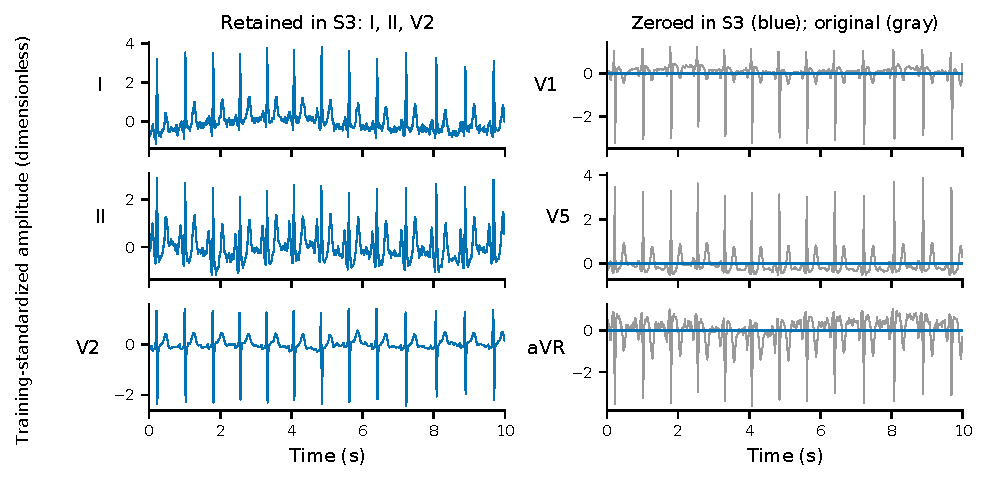
\includegraphics[width=\linewidth]{figures/input_example.pdf}
\caption{Constructing partial input from training ECG 12065 (fold 4, labelled NORM). The record is the first of a 100-record pilot sample drawn with a fixed seed from training metadata before any waveform was viewed. Six of twelve channels are shown in standardized units. S3 retains only I, II and V2; every other channel is zeroed after training-fitted standardization. Gray traces show complete-input values for three removed channels and blue lines their S3 values.}
\label{fig:input}
\end{figure}

\FloatBarrier
\section{Approach}

\subsection{Matched network and supervised intervention}

\textbf{Network.} Both arms use a residual 1D CNN with 359,749 trainable parameters, trained from scratch with PyTorch's default initialization. Its compact design permits controlled repeated training, and temporal residual CNNs have precedent in the PTB-XL benchmark \citep{strodthoff2021benchmark}. Inputs have shape 12 by 1,000. A 32-channel kernel-7, stride-1, padding-3 stem is followed by four residual blocks with widths 32/64/128/128 and first-convolution strides 1/2/2/2. Each block contains two kernel-5, padding-2 convolutions, with stride 1 in the second. All convolutions are bias-free and followed by BatchNorm1d. ReLU follows the stem, each first block convolution and each residual addition. Width or stride changes use a kernel-1 projected shortcut with BatchNorm. Global temporal average pooling and a 128-to-5 linear layer produce logits, and independent sigmoids permit co-occurring labels. The network has no additional dropout, pretraining or input augmentation. The parameters split into 2,752 for the stem, 10,368, 33,152, 131,840 and 180,992 for the four blocks, and 645 for the output layer. The receptive field is 99 samples (about 0.99\,s), enough to cover the P wave, QRS complex and T wave of one beat; the temporal length before pooling is 125, and global average pooling averages the features of all beats into one vector.

\textbf{Masking distribution.} Arm A always receives complete inputs. Arm B receives a complete input with probability 0.5; otherwise it samples a retained count $k$ uniformly from 1 through 11 and then a uniformly random subset of that size. Masks are sampled afresh at every presentation, independently of the labels, and stay constant over time; empty inputs are prohibited and targets are unchanged. Sampling the count uniformly gives every severity of missingness equal training exposure (deleting each lead independently with probability 0.5 would concentrate the retained count near six). The distribution is an engineering design that covers all severities of missingness. In practice one failed limb electrode affects several leads at once, and failures often appear as noise or a flat line; E9 partly tests these cases. The four protocol configurations can occur during training but rarely do: among 683,360 training presentations, S2, S3, S4 and S6 are expected to appear about 471, 141, 63 and 34 times.

\textbf{Relation to prior work.} The intervention builds on prior lead masking, including the self-supervised random lead masking of Oh et al., the lead-mask augmentation used by Mishra et al.\ and the lead masks of challenge entries \citep{oh2022leadagnostic,fast2026af,reyna2022issues}. We apply it in multi-label supervised learning, keep one final classifier across configurations, and add a matched control arm in which only masking is switched off. The model predicts the diagnoses directly from the retained leads; reconstruction of missing signals and an availability-indicator branch (Lecture 6, PDF p.12; video \href{https://youtu.be/AeDzGhM1GBU?t=633}{10:33}) \citep{md6329lecture06} are not used.

\textbf{Loss.} Both arms minimize unweighted binary cross-entropy with logits, averaged over records and the five targets. Standardization precedes masking, so retained channel values are unchanged by availability. The loss uses no target weighting and no inverse-keep scaling. Writing $x_{ilt}$ for the physical signal of record $i$, lead $l$ and time $t$, $m_{il}\in\{0,1\}$ for whether lead $l$ of record $i$ is available in the current presentation, and $p_{ij}=\sigma(f_\theta(\widetilde{x}_i))_j$ for the predicted probability of label $j$, the network input and training loss are
\begin{equation}
\widetilde{x}_{ilt}=m_{il}\frac{x_{ilt}-\mu_l^{\mathrm{train}}}{\max(\sigma_l^{\mathrm{train}},10^{-6})},\qquad
\mathcal{L}=-\frac{1}{5N}\sum_{i=1}^{N}\sum_{j=1}^{5}
\left[y_{ij}\log p_{ij}+(1-y_{ij})\log(1-p_{ij})\right],
\end{equation}
where the implementation uses the numerically stable logits loss. The learning rate is updated once per epoch and held constant within it. For zero-based epoch $e=0,\ldots,39$,
\begin{equation}
\eta_e=10^{-5}+\tfrac12(10^{-3}-10^{-5})\left[1+\cos(\pi e/39)\right],
\end{equation}
so the first epoch uses $10^{-3}$ and the last ($e=39$) uses $10^{-5}$.

\subsection{Training choices and validation-only selection}
\label{sec:training}

\textbf{Training and environment.} Three paired seeds, 17/29/43, share initial parameters and per-epoch record order within each A/B pair, verified by hash assertions. Masking uses an independent CPU stream seeded with seed plus 1,000,003, and epoch permutations use NumPy PCG64 SeedSequence([seed, zero-based epoch, 20261023]). All six models train for 40 epochs with batch size 64, using AdamW with initial learning rate 0.001, weight decay 0.0001 on all parameters, betas (0.9, 0.999) and epsilon $10^{-8}$. Training uses float16 CUDA autocast and dynamic gradient scaling with float32 parameters; evaluation is float32 with parameters and BatchNorm statistics frozen. Deterministic algorithms are enabled, and TF32 and cuDNN benchmarking are disabled. The software and hardware environment is PyTorch 2.6.0, CUDA 12.6 and cuDNN 9.8 on an RTX 4060 Laptop GPU; compute costs are given in Appendix~\ref{app:compute}. All code was written for this project; no course assignment code, tutorial or external repository was used as a basis. It builds on PyTorch \citep{paszke2019pytorch}, NumPy \citep{harris2020numpy}, WFDB for Python \citep{xie2023wfdb} and scikit-learn \citep{pedregosa2011sklearn}, and the presentation uses Lectrace \citep{adesanmi2026lectrace}. Code, configurations and audit records are provided in the supplementary material and at \url{https://github.com/youyang0313/ecg-lead-masking}; the presentation runs at \url{https://youyang0313.github.io/ecg-lead-masking/}.

\textbf{Hyperparameter choices.} These hyperparameters were fixed before main training without a performance grid search. The small architecture controls capacity and allows repeated training; the fixed 40-epoch budget with cosine decay is identical for both arms and controls exposure; the 50/50 mixture gives arm B equal exposure to complete and partial inputs, to protect complete-input performance (E4 later showed that higher masking ratios work better and leave complete input unaffected); and batch size 64 is a common default that an engineering trial confirmed was feasible. Arm A uses no dropout or augmentation and overfits after about epoch 11; E12 tests whether the benefit of masking comes from generic regularization.

\textbf{Checkpoint selection.} After each epoch, the checkpoint score is $0.5\,a_{\mathrm{S12}}+0.125\,(a_{\mathrm{S6}}+a_{\mathrm{S4}}+a_{\mathrm{S3}}+a_{\mathrm{S2}})$, where $a$ is validation macro-AUROC; equal scores retain the earlier epoch. Every run completes the full budget, and its selected checkpoint is used unchanged for all test configurations. Both arms use the same rule, yet its effect is asymmetric: it selects A at early epochs, before its complete-input performance peaks. E1 performs a sensitivity analysis with an S12-only rule, reported alongside the primary result in Section~\ref{sec:experiments}.

\textbf{Gen-AI contribution to method design.} The author made every method decision; the AI's role was to propose candidate analyses and find problems in the design. The author designed the shared checkpoint rule; Claude Code later found in a code review that the rule affects the two arms asymmetrically, selecting A too early, which added E1. Claude Code also proposed the mechanism ablations E2 and E7, the held-out family E8 and the fill-type stress test E9. E3, E6b, E10--E13 and the subset extension of the repair came from several rounds of simulated peer review of this paper (the academic-research-skills plugin), and the author decided case by case which to run. Some AI suggestions were modified or declined: the explicit availability indicator was demoted to an optional ablation and not run (Section~\ref{sec:ai-formulation}), and the masking-ratio sensitivity (E4), at first judged unnecessary by Claude Code, was run after review at the author's decision. All generated code was validated by paired state and order checks, checkpoint readback and independent metric checks (Section~\ref{sec:limits}), separately from any assertions generated within the code.

\subsection{Evaluation statistic and uncertainty}

\textbf{Configurations and metrics.} Configurations are S12 (all leads), S6 (I/II/III/aVR/aVL/aVF), S4 (I/II/III/V2), S3 (I/II/V2) and S2 (I/II), adapted from the challenge \citep{reyna2022issues}. For each model and configuration, macro-AUROC is the equal mean of five label AUROCs. Average precision is non-interpolated, and macro-AP likewise averages five labels. Each seed's model is evaluated separately without probability ensembling, and the primary endpoint is threshold-free.

\textbf{Primary effect and uncertainty.} The primary effect averages B-minus-A macro-AUROC over S6/S4/S3/S2 within each paired seed, then over the three seeds; complete-input change is reported separately. We use 2,000 patient bootstrap draws (seed 20261023), sharing each draw across arms, configurations and seeds and retaining every record of each sampled patient; a draw is invalid if any label lacks a positive or a negative. The resulting 95\% interval is conditional on the three trained seeds and reflects patient-level uncertainty. To reflect variation from retraining, we also report each seed's effect and a seed-based $t$ interval with two degrees of freedom.

\textbf{Decision rule.} The prespecified rule requires the lower end of the primary interval to lie above zero; it applies to the three network pairs trained here. Secondary label and configuration findings are descriptive. These rules and the six checkpoint hashes were fixed before the test labels were parsed, and the primary analysis stayed unchanged after test evaluation. Let $a^{(g)}_{r,c}$ be five-label macro-AUROC for arm $g$, seed $r$ and configuration $c$. The primary estimate is
\begin{equation}
\Delta=\frac{1}{3}\sum_{r\in\{17,29,43\}}\frac{1}{4}
\sum_{c\in\{S6,S4,S3,S2\}}\left(a^{(B)}_{r,c}-a^{(A)}_{r,c}\right).
\end{equation}

\subsection{Exploratory post-hoc analyses}
\label{sec:posthoc}

The following analyses were designed after the primary test evaluation and reuse the same test set, so all are exploratory. The primary result, the six archived checkpoints and the archived test predictions are unchanged. Every new selection uses validation data only, and every contrast uses the same 2,000-draw paired patient bootstrap (all draws valid), conditional on the trained seeds and without correction for multiple comparisons (118 intervals were computed, a few of them duplicates). Among newly trained models, E4, E7, E8 and E12 are selected by S12 validation macro-AUROC only, so held-out configurations never influence selection, and the E3 specialists are selected on their own configuration's validation data; analyses of archived models (E2, E5, E6, E6b, E9--E11, E13) report protocol-selected B and S12-selected A and B, and each contrast states the models used. Analyses are numbered in the order they were proposed; an explicit lead-availability indicator was also proposed and not run, for the reason given in Section~\ref{sec:ai-formulation}. Table~\ref{tab:analyses} summarizes the analyses.

\begin{table}[htbp]
\centering\footnotesize
\caption{Overview of the exploratory analyses. ``Both'' means protocol-selected and S12-only-selected models are reported.}
\label{tab:analyses}
\setlength{\tabcolsep}{3pt}
\begin{tabular}{L{0.7cm}L{4.3cm}L{2.2cm}L{1.6cm}L{2.5cm}L{0.9cm}}
\toprule
ID & Question & Retrained? & Selection & Main comparator & Section \\
\midrule
E1 & Is the shared selection rule unfair to either arm? & No (deterministic replay) & Both & A and B under both rules & 5.3 \\
E2 & Can test-time repairs rescue A? & No & Both & Zero-filled A & 5.4 \\
E3 & How far is one model from per-configuration specialists? & Yes (one model per configuration) & Own configuration & B under both rules, repaired A & 5.4 \\
E4 & Do results depend on the masking ratio? & Yes (masking probability 0.25/0.75/1.0) & S12 only & S12-selected A and B & 5.4 \\
E5 & Lead importance and arbitrary subsets & No & Both & A versus B & 5.5 \\
E6 & Calibration and fixed thresholds & No & Both & A versus B & 5.6 \\
E6b & Calibration of repaired A & No & Both & B & 5.6 \\
E7 & Role of the normalization layer & Yes (GroupNorm) & S12 only & S12-selected A and B & 5.4 \\
E8 & Transfer to an unseen lead family & Yes & S12 only & S12-selected B & 5.5 \\
E9 & Representation of missing leads & No & Both & Zero fill & 5.7 \\
E10 & Gap after deriving limb leads & No & Both & Zero-filled A & 5.4 \\
E11 & Strongest tested training-free repair (four configurations; extended to 207 subsets) & No & Both & Derived + re-estimated A & 5.4 \\
E12 & Is masking merely regularization? & Yes (time cutout) & S12 only & S12-selected A and B & 5.4 \\
E13 & Does B's MI output have a physiological basis? & No & S12 only (protocol also reported) & Inferior versus anterior MI & 5.5 \\
\bottomrule
\end{tabular}
\end{table}

\textbf{E1, selection sensitivity.} The shared checkpoint rule gives partial-input validation 50\% weight, which may select an early, under-trained A checkpoint. We deterministically replayed all six runs; each replayed protocol checkpoint reproduced the archived epoch and state hash exactly. During the replay we also stored the checkpoint with the best complete-input (S12) validation macro-AUROC.

\textbf{E2, test-time repairs.} Without changing any weights, we either (i) rescaled retained leads by $12/k$ for $k$ retained leads, a simple control of our own, or (ii) re-estimated every BatchNorm running mean and variance. For re-estimation, 4,096 training records drawn with a fixed seed (20261025) were masked with the target configuration; the existing running statistics were reset, and the records were passed forward in training mode in batches of 64, updating the statistics as a cumulative average (momentum set to none). This follows AdaBN with statistics from training records masked with a known configuration, so it requires knowing which leads are unavailable. We also measured, at each BatchNorm input, the absolute difference between the test-data channel mean and the running mean in units of the running standard deviation (including eps), averaged over channels.

\textbf{E3, per-configuration specialists.} For each of the four partial-input configurations we trained three models (the paired seeds, twelve models in total). Every training presentation shows only that configuration's leads, with the others zero-filled, and complete input is never shown; initialization, record order, optimizer, learning-rate schedule and precision match the formal runs. Because each specialist serves only one configuration, its checkpoint is chosen by that configuration's validation macro-AUROC, a rule more favorable to the specialists than either selection rule used for A and B. The specialists show what dedicated training attains on these fixed configurations; the selected epochs were 9--16.

\textbf{E4, masking ratio.} Arm B masks each presentation with probability 0.5. E4 changes this probability to 0.25, 0.75 and 1.0 (at 1.0, complete input is never shown in training), keeping the sampling of the retained count and subset unchanged. Each ratio is trained with the three paired seeds, with seeds, initialization, record order, mask stream, optimizer and precision matching the formal runs, selected by S12 only and compared with S12-selected A and B (ratio 0.5).

\textbf{E5, lead importance and arbitrary subsets.} Fixed models were evaluated with each lead removed in turn, with each lead retained alone, and on up to 20 random distinct subsets for each retained count $k=1,\ldots,11$ (seed 20261024). Because $k=1$ and $k=11$ admit only 12 subsets each, there are 204 random subsets, and those for $k=1$ and $k=11$ are exhaustive and coincide with the single-lead and leave-one-lead-out conditions.

\textbf{E6, calibration and operating points.} Expected calibration error is computed for each label with 15 equal-width bins and averaged over labels, a per-label adaptation of the multi-class top-label definition used by Guo et al. Per-label thresholds maximize Youden's $J$ on S12 validation predictions and are then held fixed across all test configurations, matching a deployed system that keeps its thresholds when a lead fails. E6b repeats the computation for A after the E11 repair; the repair leaves S12 input unchanged, so the thresholds are the same.

\textbf{E7, normalization ablation.} We retrained both arms with every BatchNorm1d replaced by GroupNorm with eight groups. Parameter count (359,749), convolution initialization, seeds, record order, masking and all hyperparameters are unchanged; the hyperparameters were not re-tuned for GroupNorm.

\textbf{E8, held-out lead family.} Arm B was retrained with rejection sampling so that no partial training input contains only limb leads (I, II, III, aVR, aVL, aVF). S6, S2 and every other limb-only subset are therefore unseen during training, while S4 and S3, which contain V2, belong to a seen family. A rejected draw resamples the retained count together with the subset, which slightly lowers the share of small counts (for seed 17, $k=1$ falls from 4.5\% to 2.5\% and $k=2$ from 4.6\% to 3.8\%) and makes the E8 conclusion conservative. The ``limb-only conditions'' in Section~\ref{sec:e5} are all 21 limb-only partial-input conditions evaluated in E5; the six single limb leads appear both as single-lead conditions and as $k=1$ random subsets, so they form 15 distinct subsets.

\textbf{E9, missing-lead representation.} Unavailable leads were filled with one of the following signals, in units of each lead's training standard deviation: white Gaussian noise with standard deviation 0.1 or 1.0; a sinusoidal baseline wander of amplitude 1 with frequency between 0.1 and 0.5\,Hz and random phase, drawn separately for each lead of each record; or the same lead copied from a different test record, with donors given by a fixed random permutation (seed 20261026) that never pairs a record with itself. All models received identical fill values.

\textbf{E10, derivation of missing limb leads.} All four protocol configurations contain I and II. Whenever I and II are both available, every missing limb lead is computed from them in physical units (III $=$ II $-$ I, aVR $=-$(I$+$II)/2, aVL $=$ I $-$ II/2, aVF $=$ II $-$ I/2) and standardized with the training scaler; measured leads keep their values and missing precordial leads stay zero. S4 and S3 thus both become all limb leads plus V2, S2 becomes all limb leads, and S6 is unchanged.

\textbf{E11, strongest tested training-free repair.} We combine E10's derivation with E2's BatchNorm re-estimation, re-estimating the statistics on the same 4,096 training records presented with the same derived representation. Both arms are evaluated under four conditions (zero fill, derivation only, re-estimation only, and both), to measure how much gain masked training retains over the strongest tested training-free baseline. The gaps closed by the individual repairs overlap and are not additive. We also extended this repair to every distinct partial-input subset evaluated in E5 (220 conditions, 207 distinct subsets). Whenever at least two limb leads are available, I and II are solved from them by least squares and the missing limb leads are computed; no two limb-lead axes are parallel, so any two limb leads determine the other four (relative reconstruction error 0.3\%--0.5\%). BatchNorm statistics are re-estimated separately for each subset on the same 4,096 records. Results are grouped by the number of available limb leads (fewer than two, or at least two) and by the retained count $k$; each $k$ contributes a similar number of subsets, so subset averages weight lead counts roughly equally, and we also report an average weighted by the number of subsets of each size among all 4,094.

\textbf{E12, generic augmentation control.} To test whether the benefit of masking comes from generic input-removal regularization, we trained a control arm identical to B except for how information is removed. In 50\% of presentations, $k$ is drawn uniformly from 1 to 11 and a contiguous time segment of $w=\mathrm{round}(1000\times(12-k)/12)$ samples is zeroed in all leads, starting at an integer drawn uniformly from $[0, 1000-w]$ independently for each sample. The removed fraction of the input follows the same distribution as under lead masking, and every lead remains available. Seeds, initialization, record order, optimizer and precision match the formal runs, and selection uses S12 only.

\textbf{E13, MI subclasses.} Using the MI output, we compared records with inferior MI only (PTB-XL diagnostic subclass IMI) and records with anterior MI only (AMI) separately against records without any MI and computed AUROC; the 96 records with both were excluded. This analysis is descriptive and reports no intervals.

\FloatBarrier
\section{Experiments}
\label{sec:experiments}

Sections~\ref{sec:main}--\ref{sec:labels} report the prespecified comparison; Sections~\ref{sec:e1}--\ref{sec:fill} are exploratory analyses designed after testing, which reuse the same test set without correction for multiple comparisons. We first order the evidence by strength. Against zero-filled complete-input training (A), masked training (B) gains +0.197 under the prespecified rule (+0.221 when both arms are selected on S12 only). Deriving A's missing limb leads cuts the gap to +0.104 (+0.097 under the protocol rule); adding BatchNorm re-estimation, the strongest tested training-free repair, leaves +0.017 (S12-only selection) to +0.030 (protocol rule), and the calibration gap largely disappears. Extended to 207 lead subsets, this repair matches masked training whenever at least two limb leads remain, and B's clear advantage appears on inputs with fewer than two limb leads (+0.071). Specialist models trained for each configuration exceed B by about 0.02, the price of covering every configuration with one fixed model; a generic augmentation control that removes the same amount of information as time segments gains nothing; and raising the masking ratio from 0.5 to 1.0 adds a further 0.013 on partial inputs at no complete-input cost, so the formal B is a conservative estimate. The answer to the secondary question is that most of the failure of complete-input training can be repaired without retraining, and that masked training covers any lead combination with one fixed model, clearly exceeds the repair on inputs with fewer than two limb leads, and comes within about 0.02 of a dedicated model for each configuration.

\subsection{Independent-test results}
\label{sec:main}
Table~\ref{tab:results} and Figure~\ref{fig:results} summarize the prespecified fixed-model comparison.
\begin{table}[htbp]
\centering\small
\caption{Independent-test results. A/B entries are mean $\pm$ sample SD over three seeds. Difference intervals are paired patient-bootstrap 95\% intervals conditional on these seeds. The partial mean is the prespecified primary statistic; other intervals are descriptive.}
\label{tab:results}
\begin{tabular}{lccc}
\toprule
Input & A: macro-AUROC & B: macro-AUROC & B$-$A [95\% interval] \\
\midrule
S12 & $0.9220\pm0.0059$ & $0.9282\pm0.0025$ & $+0.0062$ [0.0034, 0.0092] \\
S6 & $0.7623\pm0.0129$ & $0.8808\pm0.0012$ & $+0.1185$ [0.1084, 0.1287] \\
S4 & $0.7273\pm0.0401$ & $0.9023\pm0.0005$ & $+0.1751$ [0.1647, 0.1856] \\
S3 & $0.7016\pm0.0330$ & $0.8959\pm0.0032$ & $+0.1942$ [0.1827, 0.2064] \\
S2 & $0.5718\pm0.0769$ & $0.8738\pm0.0022$ & $+0.3020$ [0.2897, 0.3150] \\
\midrule
Partial mean & $0.6908\pm0.0391$ & $0.8882\pm0.0017$ & $+0.1974$ [0.1882, 0.2067] \\
\bottomrule
\end{tabular}
\end{table}

\begin{figure}[htbp]
\centering
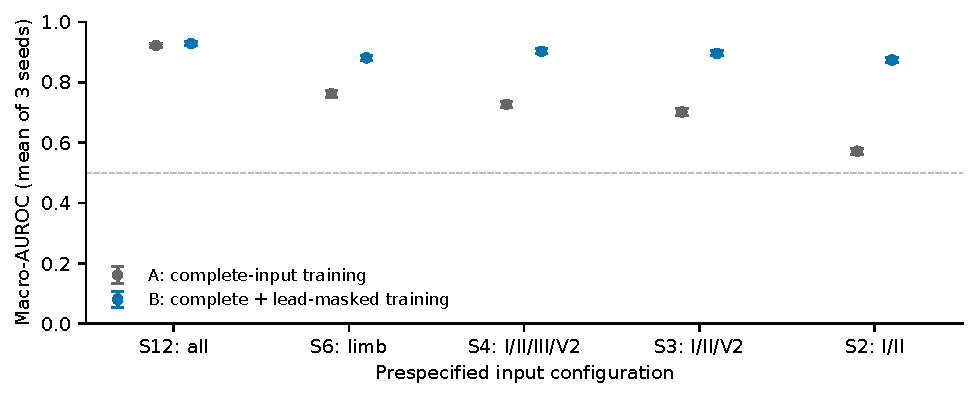
\includegraphics[width=\linewidth]{figures/test_discrimination.pdf}
\caption{Independent-test macro-AUROC for each input configuration (2,158 recordings, 1,877 patients). Points average three separately trained seeds; bars are descriptive patient-bootstrap 95\% intervals conditional on those seeds and are barely visible because the intervals are narrow. Table~\ref{tab:results} reports seed SD. The dashed line at 0.5 marks chance. S6 and S4 change lead identity as well as count, so the categories are not a lead-count dose response.}
\label{fig:results}
\end{figure}

All six fixed models were evaluated on the same 2,158 recordings from 1,877 held-out patients. Mean partial-input macro-AUROC was 0.6908 for A and 0.8882 for B. The prespecified paired effect was +0.1974 AUROC units, with 95\% patient-bootstrap interval [0.1882, 0.2067]; all 2,000 draws were valid. The positive lower endpoint supports the primary hypothesis under the prespecified rule. The effect is measured in AUROC units and is the gain over zero-filled complete-input training; gains over stronger baselines are reported in Section~\ref{sec:mechanism}.

For seeds 17/29/43, paired effects were +0.1800/+0.2423/+0.1701 (sample SD 0.0391); every seed favored B, with varying magnitude. Partial-input mean AUROC had seed SDs of 0.0391 for A and 0.0017 for B. Uncertainty from retraining is reflected by the seed-based $t$ interval (two degrees of freedom), [0.100, 0.295], about ten times wider than the patient interval, with a lower endpoint well above zero.

Complete-input macro-AUROC was 0.9220 for A and 0.9282 for B, a paired difference of +0.0062 with descriptive patient interval [0.0034, 0.0092]; complete-input macro-AP was 0.8120/0.8263. Section~\ref{sec:e1} (E1) tests whether this small advantage comes from the shared selection rule.

Gains per partial configuration were +0.1185 (S6), +0.1751 (S4), +0.1942 (S3) and +0.3020 (S2), and macro-AP improved in every configuration, from 0.5633/0.5269/0.4946/0.3618 to 0.7291/0.7716/0.7602/0.7157. Table~\ref{tab:results} reports all four configurations, which also provide an internal check. By design, S2 and S6, and S3 and S4, are approximately equivalent in information, because the remaining limb leads are linear combinations of I and II \citep{reyna2022issues}. B respects this equivalence (S6/S2 0.881/0.874, S4/S3 0.902/0.896), whereas A drops by 0.19 from S6 to S2. The complete-input model therefore did not use the linear redundancy; Section~\ref{sec:mechanism} shows that it can be used through explicit derivation.

\subsection{Label behavior and interpretation of the baseline drop}
\label{sec:labels}

The largest average gain occurred for I/II inputs. Under S2, A/B label AUROCs were NORM 0.5707/0.9123, MI 0.5336/0.8348, STTC 0.6727/0.9047, CD 0.6817/0.8871 and HYP 0.4003/0.8300. Benefits involved several labels with heterogeneous magnitudes. A's HYP AUROC of 0.40 is clearly below chance, which indicates a systematically inverted ranking; this agrees with the sharp rise in A's positive-prediction rate under missing leads (Section~\ref{sec:calibration}). B's S2 macro-AUROC remained below its complete-input value, so additional leads still carry information. These are descriptive results.

Under zero-filling, A reached 0.9220 on complete inputs and 0.6908 averaged over partial inputs, whereas B reached 0.8882 from exactly the same retained signals. Absent information alone cannot explain A's full deterioration. Section~\ref{sec:mechanism} shows that most of it stems from inconsistent zero-filled inputs and shifted activation statistics, which can be repaired at test time. The independent-test pattern resembles the development means of 0.6861/0.8906; the hypothesis was tested on test results.

\subsection{Selection sensitivity (E1)}
\label{sec:e1}

\begin{figure}[htbp]
\centering
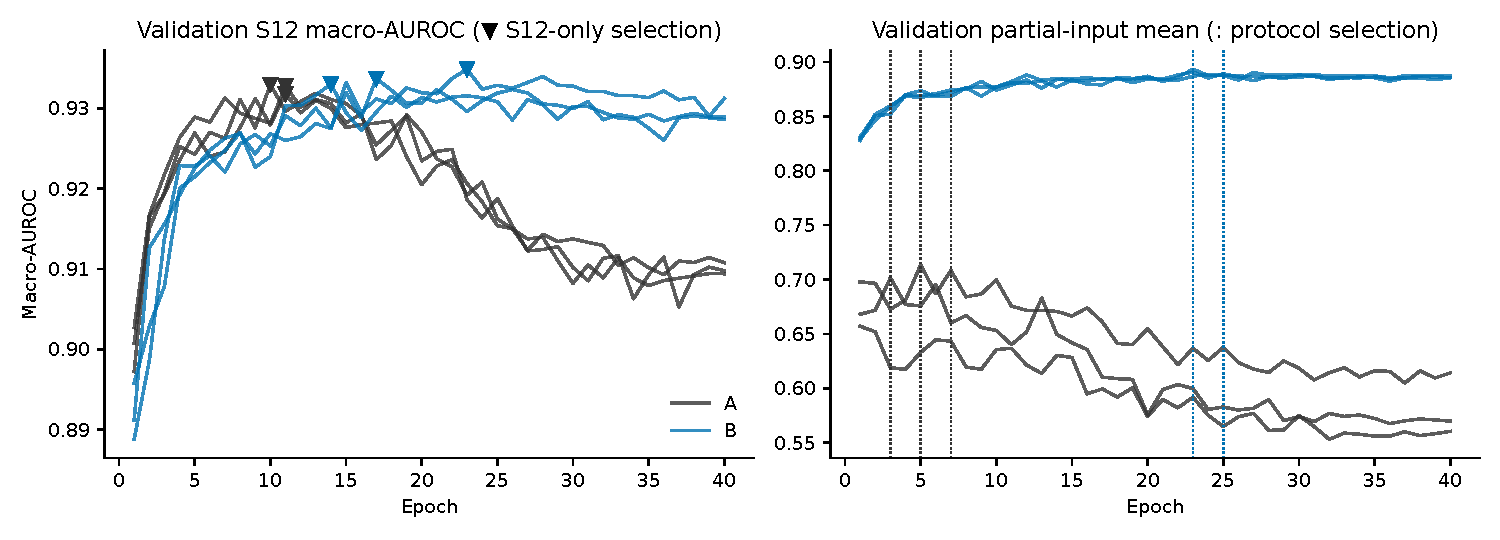
\includegraphics[width=\linewidth]{figures/e1_validation_trajectories.pdf}
\caption{Validation trajectories from the deterministic replay of all six runs. Left: complete-input macro-AUROC; triangles mark the checkpoints chosen by S12-only selection. Right: mean over the four partial configurations; dotted vertical lines mark the epochs chosen by the protocol rule (two of B's three coincide at epoch 23). A's partial-input performance declines steadily while it trains, and A overfits on complete input after about epoch 11. B is stable on both.}
\label{fig:e1}
\end{figure}

Under S12-only selection, A is selected at epochs 11/11/10 rather than 3/7/5, and B at 17/14/23. A's complete-input test AUROC improves by +0.0054 [0.0034, 0.0075] to 0.9273, so the B$-$A complete-input difference falls to +0.0010 [$-$0.0010, 0.0031]. The small complete-input advantage in Section~\ref{sec:main} therefore comes mostly from the shared selection rule, and the two arms are comparable on complete input. Meanwhile, A's partial-input mean falls to 0.6637 and the B$-$A partial-input gain widens to +0.2210 [0.2120, 0.2303] (both arms S12-selected). Figure~\ref{fig:e1} explains why: under zero-filling, the longer A trains, the lower its partial-input validation AUROC, which drifts from about 0.70 to 0.57. The primary effect is therefore larger under S12-only selection. This pattern is specific to zero-filling: after the E11 repair, the longer-trained A is better (0.868 under S12-only selection, 0.858 under the protocol rule; Section~\ref{sec:mechanism}).

\subsection{Why does complete-input training fail, and how much does masking add? (E2, E3, E4, E7, E10--E12)}
\label{sec:mechanism}

\begin{table}[htbp]
\centering
\caption{Repair ladder. Test macro-AUROC per partial-input configuration (mean over three seeds) of S12-selected models (except the specialists), the share of the zero-filled A gap that each row closes, and paired patient-bootstrap 95\% intervals for B (zero-fill) minus each row. Shares come from different single repairs, overlap and are not additive. Specialists are one model per configuration, each selected on its own configuration's validation data.}
\label{tab:ladder}
\footnotesize\setlength{\tabcolsep}{3.5pt}
\begin{tabular}{lccccccc}
\toprule
Model and test-time handling & S6 & S4 & S3 & S2 & Partial mean & Gap closed & B $-$ row [95\% interval] \\
\midrule
A, zero-fill & 0.745 & 0.709 & 0.684 & 0.517 & 0.664 & --- & +0.221 [0.212, 0.230] \\
A, GroupNorm retrained (E7) & 0.762 & 0.792 & 0.782 & 0.727 & 0.766 & 46\% & +0.119 [0.113, 0.125] \\
A, derived limb leads (E10) & 0.745 & 0.816 & 0.816 & 0.745 & 0.781 & 53\% & +0.104 [0.095, 0.113] \\
A, BatchNorm re-estimated (E2) & 0.846 & 0.859 & 0.862 & 0.783 & 0.837 & 79\% & +0.047 [0.042, 0.053] \\
A, derived + re-estimated (E11) & 0.846 & 0.889 & 0.889 & 0.846 & 0.868 & 92\% & +0.017 [0.011, 0.023] \\
Time-cutout control (E12) & 0.742 & 0.712 & 0.681 & 0.480 & 0.654 & $-$5\% & +0.231 [0.222, 0.240] \\
B, zero-fill & 0.880 & 0.899 & 0.891 & 0.868 & 0.885 & --- & --- \\
Specialists (E3, 12 models) & 0.897 & 0.915 & 0.913 & 0.895 & 0.905 & 109\% & $-$0.020 [$-$0.024, $-$0.016] \\
\bottomrule
\end{tabular}
\end{table}

\textbf{Activation statistics and test-time re-estimation (E2).} Zero-filling leads shifts the activation statistics inside the network. Excluding the stem, where zero-mean standardized inputs leave the mean unchanged, the S2 input mean at the BatchNorm layers of S12-selected A deviates from the running mean by 0.24--0.46 running SDs, compared with at most 0.06 under S12; S12-selected B deviates less (0.09--0.24). Re-estimating the BatchNorm statistics under the target mask, without changing any weight, raises A's partial-input mean from 0.664 to 0.837 (Table~\ref{tab:ladder}), closing about 79\% of the gap (77\% relative to protocol-selected B). Rescaling the retained leads by $12/k$, which does not touch BatchNorm, recovers +0.135 (about 61\%). The same re-estimation changes protocol-selected B only slightly ($-$0.003 [$-$0.005, $-$0.0005]), consistent with B's statistics having been estimated on mini-batches that already mix complete and masked samples.

\textbf{Normalization ablation (E7).} Replacing BatchNorm with GroupNorm, which normalizes each record separately, and retraining raises A's partial-input mean by +0.102, about 46\% of the gap, without any test-time adaptation (Appendix Figure~\ref{fig:e8}). GroupNorm A remains 0.119 [0.114, 0.125] below GroupNorm B, and its partial-input validation performance also declines during training (Appendix Figure~\ref{fig:e8dyn}). With masked training, the normalization choice makes no visible difference (+0.0003 [$-$0.004, 0.004]). Untuned GroupNorm lowers complete-input AUROC by about 0.015 in both arms ($-$0.0155 [$-$0.0199, $-$0.0113] for A), so we use it as mechanism evidence.

\textbf{Lead derivation (E10).} Much of A's collapse under S2 comes from the input itself: III, aVR, aVL and aVF are exact functions of I and II, and zero-filling presents inputs that contradict this relation. Deriving the missing limb leads raises A's partial-input mean from 0.664 to 0.781; after derivation the S2 input equals the full limb-lead set, so its score equals that of S6 (0.745). The B$-$A gap falls from +0.221 to +0.104 (for protocol-selected models, from +0.197 to +0.097 [0.088, 0.106]). Derivation changes B little (+0.004 under the protocol rule, +0.007 under S12-only selection), indicating that B had already learned to use the redundancy. The gap remaining after derivation lies in configurations that lack precordial leads, and most of it can be closed further by BatchNorm re-estimation.

\textbf{Strongest tested training-free repair (E11).} Combining derivation with BatchNorm re-estimation raises A's partial-input mean to 0.868, closing about 92\% of the gap (85\% under the protocol rule); B still leads by +0.017 [0.011, 0.023] (+0.015, +0.016 and +0.020 for the three seeds; seed $t$ interval [0.011, 0.023]), and by +0.030 [0.024, 0.037] for protocol-selected models (seed $t$ interval [0.019, 0.042]). When B receives the same repair, it still leads by +0.024 [0.019, 0.029] (+0.031 [0.025, 0.036] under the protocol rule). The repairs depend on the order in which they are applied: derivation alone closes about 53\%, and re-estimation after derivation adds about 39\%. Overall, recalibrating the network's internal activations per configuration (BatchNorm re-estimation or, to a lesser degree, $12/k$ rescaling) recovers most of the gap, consistent with a BatchNorm statistic mismatch. The remaining gap lies mainly on the limb-only configurations S6 (+0.034) and S2 (+0.022); S4 and S3, which include V2, show +0.010 and +0.002.

\textbf{Per-configuration specialists (E3).} To measure how much a fixed model gives up against dedicated training, we trained a separate model for each partial-input configuration that only ever sees that configuration (four configurations $\times$ three seeds), each selected on its own configuration's validation AUROC, a rule that favors the specialists over B. The specialists reach a partial-input mean of 0.905, exceeding S12-selected B by +0.020 [0.016, 0.024] (seed $t$ interval [0.009, 0.031]; protocol-selected B: +0.017 [0.013, 0.020]) and the strongest tested repair by +0.037 [0.032, 0.043]. All three seeds agree in direction, and the difference from B lies between +0.012 and +0.027 in every configuration. The specialists also respect the approximate S6/S2 and S4/S3 equivalence (0.897/0.895 and 0.915/0.913). On the four protocol configurations, B therefore lies between the strongest training-free repair (0.868) and the specialists (0.905): covering any lead combination with one fixed model costs about 0.02 relative to a dedicated model for each configuration.

\begin{figure}[htbp]
\centering
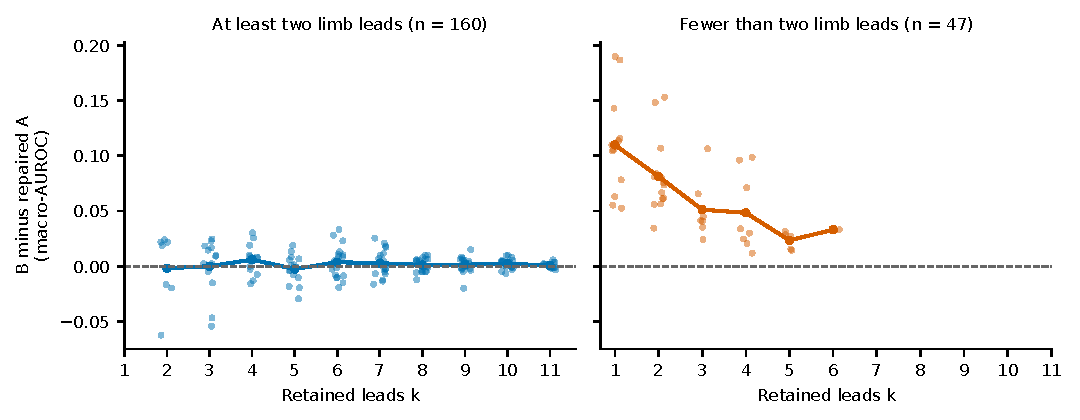
\includegraphics[width=0.95\linewidth]{figures/e12_subset_gap.pdf}
\caption{B (zero-fill) minus E11-repaired A in test macro-AUROC across 207 lead subsets, by retained count $k$, for subsets with at least two limb leads (left, 160 subsets) and fewer than two (right, 47 subsets). S12-only selection, means over three seeds; points are subsets, lines are means per $k$, and the dashed line marks zero.}
\label{fig:subsets}
\end{figure}

\textbf{The repair across arbitrary lead subsets (E11 extension).} The four protocol configurations all keep at least two limb leads and at most one precordial lead. To test whether the conclusions extend to other lead combinations, we applied the E11 repair to all 207 distinct partial-input subsets evaluated in E5 (Figure~\ref{fig:subsets}). On average, B leads repaired A by +0.018 [0.015, 0.021] (+0.022 [0.019, 0.025] under the protocol rule), and the repair closes 85\% of the gap. The gap comes almost entirely from the 47 subsets with fewer than two limb leads, where derivation is impossible: there B leads by +0.071 [0.067, 0.076], and by +0.110 [0.104, 0.116] for single leads. Whenever at least two limb leads remain (160 subsets), the two are effectively tied (+0.002 [$-$0.002, 0.005]; +0.009 under the protocol rule), with gaps between $-$0.002 and +0.006 at every lead count. The protocol configurations show a larger gap (+0.017) because S6 and S2 contain only limb leads. Each lead count contributes a similar number of subsets; weighting lead counts by their frequency among all 4,094 subsets gives an average gap of about +0.008. Applying the same repair to B helps slightly across all subsets (0.896 versus 0.892) and hurts slightly on subsets with fewer than two limb leads (0.838 versus 0.849).

\textbf{Implications for deployment.} All three approaches first require identifying which leads are unavailable (Section~\ref{sec:fill}). They differ in what must be maintained and in which inputs they suit. Specialists need one model per lead configuration and perform best on the four protocol configurations. The strongest tested repair needs no retraining, but the deployment site must keep training data, or precompute and manage one set of BatchNorm statistics for every configuration that may occur, and derivation works only when at least two limb leads remain: on inputs with precordial leads it matches B, with limb leads only (as on a handheld six-lead device, S6) it trails by about 0.03, and with fewer than two limb leads it trails by about 0.07 on average. B is one fixed model with one set of thresholds, covers any lead combination and keeps its calibration (Section~\ref{sec:calibration}), at a cost of about 0.02 relative to dedicated models. In practice, a dedicated model suits a fixed configuration when retraining is possible; masked training suits unpredictable lead combinations; and when only an existing complete-input model is available, derivation with re-estimation suits inputs that contain precordial leads and at least two limb leads.

\textbf{Generic augmentation control (E12).} Finally, we test whether the benefit of masking comes from generic regularization. The control arm removes the same fraction of information as B, as a time segment across all leads. On complete input, no difference from A or B was observed (absolute differences at most 0.002). On partial inputs it gains nothing: its partial-input mean is 0.654, $-$0.010 relative to A (patient interval [$-$0.015, $-$0.006]; the three seeds disagree in sign and the seed $t$ interval is [$-$0.082, +0.062]), and B exceeds it by +0.231 [0.222, 0.240]. Removing the same fraction of information as time segments does not reproduce the benefit of masked training.

\textbf{Masking ratio (E4).} Higher masking ratios work better. With masking probabilities of 0.25, 0.5, 0.75 and 1.0, the partial-input means are 0.873, 0.885, 0.893 and 0.898; relative to 0.5, a ratio of 1.0 adds +0.013 [0.011, 0.015] (positive for all three seeds), and 0.25 loses $-$0.012 [$-$0.014, $-$0.010]. Complete input shows no cost: even when complete input is never shown in training (ratio 1.0), complete-input AUROC is 0.9285, +0.0001 [$-$0.0016, 0.0019] relative to 0.5, possibly because masked inputs that keep 10--11 leads are already close to complete. The concern about complete-input performance behind the 50/50 choice (Section~\ref{sec:training}) is therefore unnecessary here, and the formal B is a conservative estimate: trained at a ratio of 1.0, its lead over the strongest tested repair grows from +0.017 to about +0.030, and its gap to the specialists shrinks from 0.020 to about 0.007. These comparisons use S12-only selection; the ratio was changed after seeing test results, so the finding is exploratory.

\subsection{Lead importance, unseen lead families and MI subclasses (E5, E8, E13)}
\label{sec:e5}

\begin{figure}[htbp]
\centering
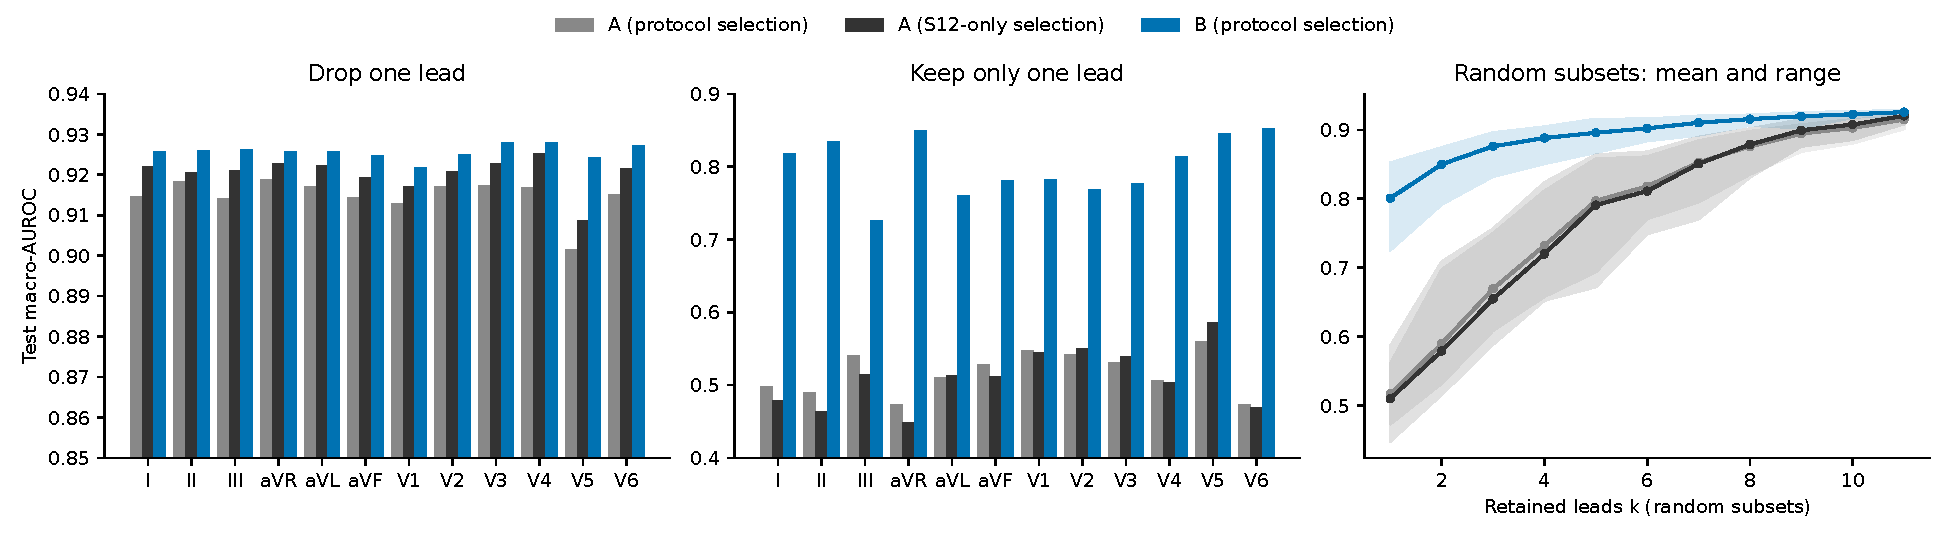
\includegraphics[width=\linewidth]{figures/e6_lead_importance.pdf}
\caption{Fixed-model test macro-AUROC when one lead is removed (left; the axis starts at 0.85 and magnifies differences of about 0.01), when only one lead is retained (middle), and on 204 random subsets by retained count (right; line = mean, band = range). Means over three seeds.}
\label{fig:e6}
\end{figure}

\textbf{Lead importance and arbitrary subsets (E5).} Here S12-selected A is compared with protocol-selected B (S12-selected B is similar). Removing any single lead barely affects either arm (A 0.909--0.925, B 0.922--0.928; Figure~\ref{fig:e6}); a removed limb lead can always be reconstructed from the remaining limb leads, so leave-one-out cannot reveal limb-lead importance. With a single retained lead, zero-filled A is near or below chance (0.45--0.59), while B reaches 0.73--0.85, best with V6, aVR, V5 and II and worst with III (0.726). Per-label single-lead results (Appendix Figure~\ref{fig:e6label}) are strongest for NORM and STTC and weaker for MI and HYP. Across random subsets, B with one lead (0.80) is comparable to zero-filled A with five or six leads (0.79--0.81), and B's worst subset at every count exceeds zero-filled A's mean. Most of the 204 subsets are not protocol configurations, so the benefit extends beyond the four reported sets.

\textbf{Held-out lead family (E8).} Because evaluation configurations could occur during B's training, E8 retrained B without any limb-only partial input (S12-only selection, compared with S12-selected B). On the held-out S6/S2, this model is 0.0044 [0.0017, 0.0075] below B and 0.239 [0.229, 0.249] above zero-filled A; on the seen family (S4/S3) and on complete input, no difference was observed ($-$0.0010 and +0.0008, both intervals including zero). Averaged over the 21 limb-only conditions evaluated in E5 (15 distinct subsets; Section~\ref{sec:posthoc}), it reaches 0.801, versus 0.815 for B and 0.522 for zero-filled A (Appendix Figure~\ref{fig:e9}), with larger drops for the single leads III and aVL (about 0.03--0.04). Masked training therefore transfers to limb-only combinations never seen in training, at a cost of about 0.015, smaller than B's advantage over the strongest tested repair on such subsets (+0.044 on the 15 limb-only subsets; Section~\ref{sec:mechanism}). E8 held out one lead family.

\textbf{MI subclasses (E13).} To check whether B's MI output from few leads has a physiological basis, we used it to separate records with inferior MI only (231) or anterior MI only (210) from records without any MI (1,608); records with both (96) were excluded. With limb leads only, B detects inferior MI clearly better than anterior MI (S12-selected B: 0.886 versus 0.788 under S6, 0.828 versus 0.787 under S2). Once the precordial lead V2 is added, anterior MI rises to 0.92--0.93 (0.917 under S4, 0.931 under S3). This matches the anatomical coverage of the leads: inferior MI appears in II, III and aVF, and anterior MI mainly in the precordial leads. B's few-lead MI output thus reflects the location of the infarction. Zero-filled A is near or below chance for both subclasses under S2 (0.38 and 0.49). PTB-XL's MI labels come from infarction statements in the reports, which is a different task from acute MI triage.

\subsection{Calibration and fixed operating thresholds (E6)}
\label{sec:calibration}

\begin{figure}[htbp]
\centering
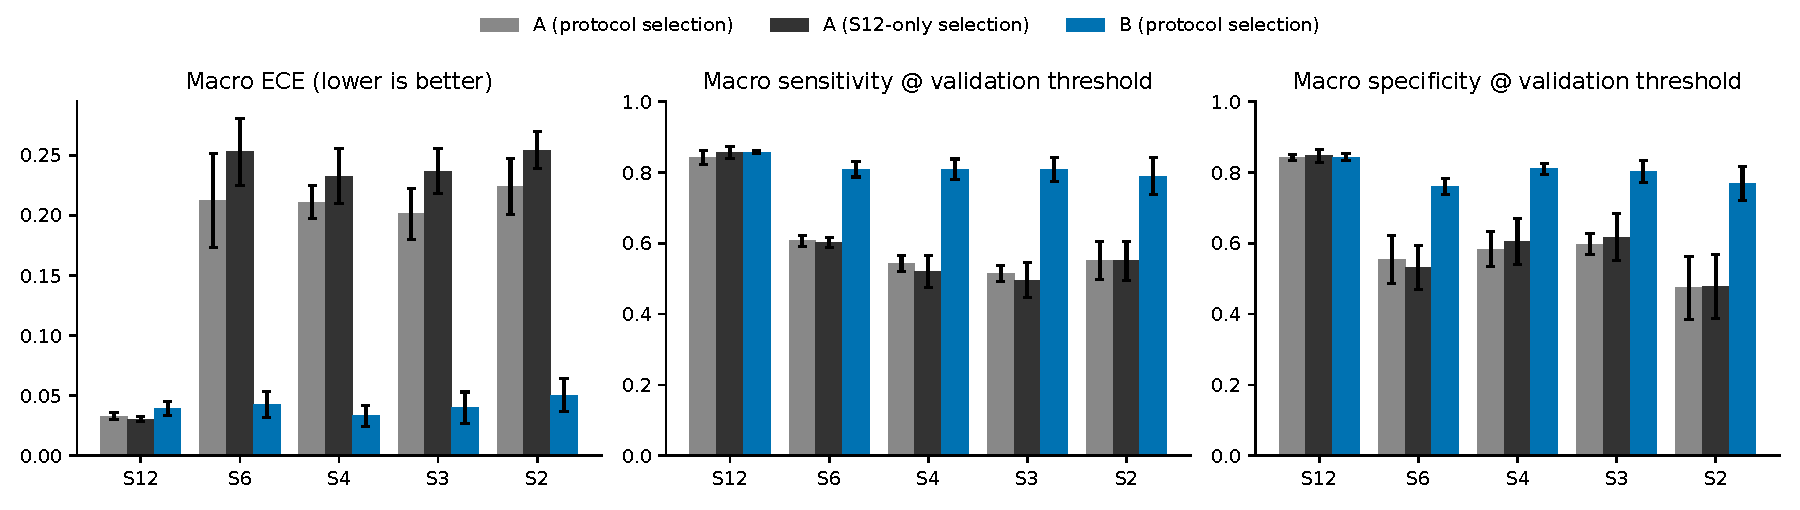
\includegraphics[width=\linewidth]{figures/e7_calibration_thresholds.pdf}
\caption{Macro expected calibration error (left) and macro sensitivity/specificity at per-label thresholds chosen on S12 validation predictions and held fixed across configurations (middle, right). Mean $\pm$ seed SD.}
\label{fig:e7}
\end{figure}

Whether probabilities and thresholds keep their meaning needs checking beyond AUROC. Under missing leads, zero-filled A's macro ECE (under either selection rule) rises from 0.03 on complete input to 0.20--0.25 (Figure~\ref{fig:e7}). At its validation thresholds, its macro sensitivity falls to 0.50--0.61 and specificity to 0.47--0.62, and under S2 its positive-prediction rate rises from 0.34 to 0.53. B keeps ECE at 0.03--0.06, sensitivity at 0.74--0.81 and specificity at 0.76--0.83 (ranges over both selection rules).

\textbf{Calibration of repaired A (E6b).} Most of the calibration and threshold collapse can also be repaired. After E11's derivation and BatchNorm re-estimation, with thresholds unchanged, A's ECE falls to about 0.06 under both S6 and S2, its positive-prediction rate returns to 0.33--0.34, and its sensitivity and specificity are about 0.70--0.71 and 0.80--0.81 (similar under both selection rules). S12-selected B has ECE 0.058/0.051, sensitivity 0.76/0.74 and specificity 0.77/0.81 under S6/S2. The two differ in ECE by at most 0.01; B's sensitivity is 0.03--0.06 higher, its specificity is 0.03 lower under S6 and similar under S2, and its sum of sensitivity and specificity is 0.03--0.04 higher, consistent with the remaining AUROC gap. With the same repair, B reaches ECE 0.043 under S6/S2 and a sum of sensitivity and specificity about 0.07 above repaired A. For a system with fixed thresholds, the key is to avoid using an unrepaired complete-input model directly; after repair, A and B are similarly calibrated.

\subsection{Representation of unavailable leads (E9)}
\label{sec:fill}

\begin{table}[htbp]
\centering\small
\caption{Partial-input mean test macro-AUROC when unavailable leads are filled with alternative signals instead of zero. Units are training standard deviations of each lead. A and B use different selection rules (a mixed pairing that favors B). GN: GroupNorm.}
\label{tab:fill}
\begin{tabular}{lccccc}
\toprule
Model & Zero & Noise $\sigma{=}0.1$ & Baseline wander & Noise $\sigma{=}1$ & Other record's lead \\
\midrule
A (S12-selected) & 0.664 & 0.664 & 0.671 & 0.591 & 0.585 \\
B (protocol) & 0.888 & 0.885 & 0.869 & 0.684 & 0.653 \\
GN B (S12-selected) & 0.885 & 0.880 & 0.857 & 0.699 & 0.624 \\
\bottomrule
\end{tabular}
\end{table}

All previous results assume that unavailable leads are detected and zeroed. B tolerates low-amplitude noise and baseline wander ($-$0.003 and $-$0.020), and signal-like corruption degrades it sharply (Table~\ref{tab:fill}). Typical-amplitude white noise ($\sigma=1$, a crude proxy for poor electrode contact) costs $-$0.204 [$-$0.213, $-$0.196], and a plausible ECG copied from another record, a signal-level stress test, costs $-$0.235 [$-$0.250, $-$0.221]. B remains better than zero-filled A under every fill (+0.093 and +0.068 for the two hardest), with its advantage reduced by about 59\%--70\% relative to zero-filling. B has learned to ignore zeroed channels; plausible-looking wrong signals have to be identified and zeroed by an upstream lead-quality or electrode-contact check.

\subsection{Reliability, limitations and AI-supported workflow}
\label{sec:limits}

\textbf{Reliability.} An evaluation reimplemented by Codex in scikit-learn, separate from the pipeline's weighted-AUROC implementation, reproduced all 300 test AUROC/AP values. For the exploratory analyses, the deterministic replay reproduced all six archived checkpoint hashes, and re-running the archived models reproduced the archived test predictions exactly. Appendix~\ref{app:compute} gives the full verification and compute record.

\textbf{Limitations.} The study uses one public cohort, one backbone and three seeds, with fixed rather than searched hyperparameters (including for GroupNorm). The analyses in Sections~\ref{sec:e1}--\ref{sec:fill} were designed after the primary test evaluation and reuse the same test set; the selections they involve use validation data only, and the results are exploratory. E5 and E8 extend evaluation beyond the four protocol sets; E5's leave-one-out is confounded by limb-lead redundancy and cannot reveal limb-lead importance; E8 held out one lead family; the E3 specialists cover only the four protocol configurations; and the strongest tested repair does not include reconstruction methods such as regressing missing precordial leads on the available ones. We did not test an explicit availability indicator, and the 100\,Hz release may limit fine morphological detail for both arms. Digital removal does not reproduce device-specific acquisition changes or the effect of a detached limb electrode on all precordial leads through the Wilson central terminal, and E9 shows that robustness depends on unavailable leads being detected and zeroed. We did not perform per-record error analysis, per-label operating points (such as sensitivity at fixed specificity, or PPV/NPV at realistic prevalence) or subgroup analyses by age or sex, and there was no external validation and no evaluation of clinical outcomes; the thresholds in E6 illustrate operating behaviour. Lecture 11's robustness discussion (PDF p.40; video \href{https://youtu.be/DDU159QXVzI?t=1735}{28:55}) applies directly: trust claims must match the tested changes in setting \citep{md6329lecture11}.

\textbf{Role of AI in coding and experimental evaluation.} OpenAI Codex wrote and debugged the main pipeline, identified failure modes, recovered logging and reimplemented the scikit-learn check above; Claude Code organized audit records, drafted figures and text, and prompted distinctions between validation and testing, patient-level and seed-level uncertainty, and ranking scores and clinical decisions. The exploratory analyses were implemented as separate scripts that do not modify the archived pipeline; their origins are listed in Section~\ref{sec:posthoc} and the method-design paragraph of the Approach. The multi-round simulated peer review had the largest effect on the evaluation: the stronger baselines it proposed placed B's advantage over the strongest baseline at +0.017--0.030 on the protocol configurations and showed that this advantage is concentrated on inputs with fewer than two limb leads, while the prespecified primary effect is unchanged. The AI also makes errors that need checking. Its draft methods text gave 220 random subsets for E5 (actually 204) and described a $-$0.003 difference as ``smaller than the variation between seeds'' (it exceeds protocol-selected B's seed SD). More importantly, the first version of the subset extension derived limb leads only when I and II were both present, although any two limb leads suffice; this implementation limit nearly doubled B's apparent advantage across arbitrary subsets (+0.034 versus the corrected +0.018). All three were found when a later round of simulated review checked the text against the code and result files. The author decided which suggestions to run and how to interpret the results.

\section{Conclusion}

\textbf{Key findings.} In a matched comparison, mixing complete inputs with random whole-lead masking raised a fixed classifier's mean macro-AUROC over four predefined partial-input conditions from 0.6908 to 0.8882 (+0.1974, [0.1882, 0.2067]); under complete-input-only selection, no complete-input difference was observed. This gain is measured against a zero-filled baseline, and the exploratory analyses place it more precisely. Inconsistent zero-filled inputs and shifted activation statistics are the main cause of the failure: on the four protocol configurations, deriving the missing limb leads and re-estimating BatchNorm statistics repairs 85\%--92\% of the gap without retraining, masked training exceeds this repair by 0.017--0.030, and it is about 0.02 below models trained for each configuration. Across 207 lead subsets, the repair matches masked training whenever at least two limb leads remain (+0.002); with fewer than two limb leads masked training leads by 0.071, and by 0.110 for single leads. A time-cutout control that removes the same amount of information gains nothing. Higher masking ratios work better: masking every presentation adds a further 0.013 on partial inputs with no complete-input loss. Masked training transfers to a withheld limb-only lead family, and its MI output agrees with the anatomical coverage of the leads.

\textbf{Implications for deployment.} All three approaches need upstream identification of unavailable leads, because signal-like corruption removes most of the advantage of masked training (E9). Given that, the choice depends on the input. For unpredictable lead combinations, one masked-training model covers any combination without per-configuration statistics and on average exceeds the strongest tested repair. For a device with one fixed lead configuration, where retraining is possible, a dedicated model is better. When only an existing complete-input model is available, derivation with per-configuration BatchNorm re-estimation comes close to masked training on inputs with at least two limb leads and some precordial leads, trails by about 0.03 with limb leads only (as on a handheld six-lead device, S6), and trails by about 0.07 on average with fewer than two limb leads.

\textbf{What we learned.} The clearest lesson of this project is that the size of an effect depends on the baseline it is measured against: the same intervention gains +0.197 over a zero-filled baseline, +0.017--0.030 over the strongest tested training-free repair on the protocol configurations, close to zero on subsets with at least two limb leads, and a clear margin with fewer than two. Robustness studies should report cheap strong baselines first and test beyond the protocol configurations. A shared selection rule applied to a flawed input representation can pick an under-trained checkpoint for the baseline: under zero-filling, the longer A trains, the worse its partial-input performance (E1), while after repair the longer-trained A is better, which raises B's lead under the protocol rule from +0.017 to +0.030. With AI assistance, the same kind of tool gives different results in different roles. When it only checked claims already written, it missed important precedents and stronger baselines; when asked to search for missing baselines as a reviewer would, it found them and still missed things: one round of simulated review proposed the calculation that any two limb leads determine the others, without noticing that our subset extension derived leads only from I and II, which the next round caught. Reliable conclusions came from several rounds of adversarial checking and from checking every claim against the code and result files.

\textbf{Limitations and future work.} The study uses one public cohort, one backbone and three seeds; the exploratory analyses reuse the same test set, and about 120 intervals were not corrected for multiple comparisons. Lead loss is simulated digitally and completely at random, without device-specific acquisition differences or electrode faults; for example, a detached limb electrode also changes the Wilson central terminal (defined in \citep{reyna2022issues}) and so affects all precordial leads. The specialists cover only the four protocol configurations, E8 held out one lead family, and the strongest tested repair excludes reconstruction methods such as regressing missing precordial leads. Labels stop at diagnostic superclasses, and the sampling rate is 100\,Hz. Future work includes external validation on the multi-centre PhysioNet/CinC 2021 data and on real six-lead and two-lead devices; simulating faults per electrode and combining the model with lead-quality detection; testing whether the remaining gap comes from cross-lead features; and evaluation on finer diagnostic statements and clinical operating points (sensitivity at fixed specificity, PPV/NPV at realistic prevalence). Clinical use requires further decision-level validation.

\begingroup
\interlinepenalty=10000
\bibliographystyle{abbrvnat}
\bibliography{references}
\endgroup
% v9.5 appendix (2026-10-25): analyses numbered E1--E13; E2 and E9 figures removed (values in tab:ladder and tab:fill).
\clearpage
\appendix
\section{Supplementary exploratory figures}

All figures in this appendix come from the exploratory analyses described in Section~\ref{sec:posthoc}. They use S12-only checkpoint selection unless stated otherwise, show means over three seeds, and use the same independent test set as the main results. Source code is in \texttt{posthoc/} and outputs are in \texttt{experiments/posthoc/} of the supplementary material; script and folder names there use the original proposal numbers, and the supplementary README maps them to E1--E13.

\begin{figure}[htbp]
\centering
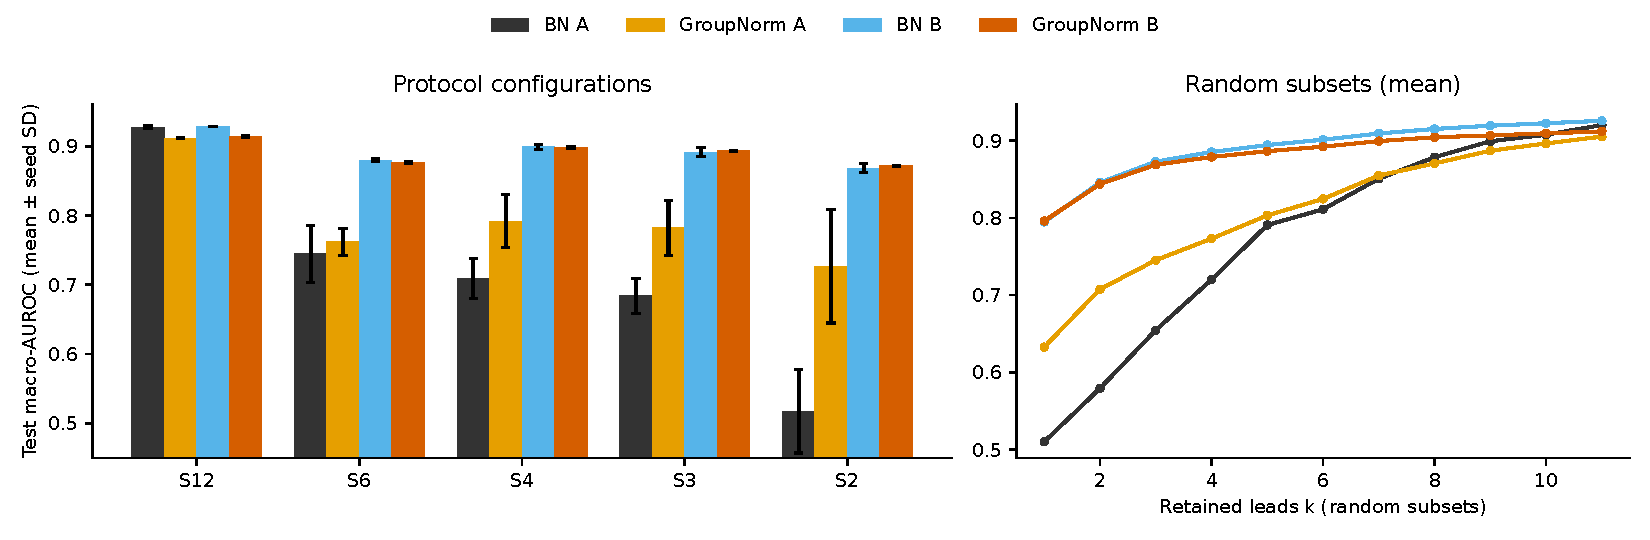
\includegraphics[width=\linewidth]{figures/e8_normalization_ablation.pdf}
\caption{E7: BatchNorm versus GroupNorm(8) for both arms. Left: protocol configurations (mean $\pm$ seed SD). Right: mean over random subsets by retained count. GroupNorm improves complete-input training under missing leads, stays below masked training, and costs about 0.015 complete-input AUROC without re-tuning.}
\label{fig:e8}
\end{figure}

\begin{figure}[htbp]
\centering
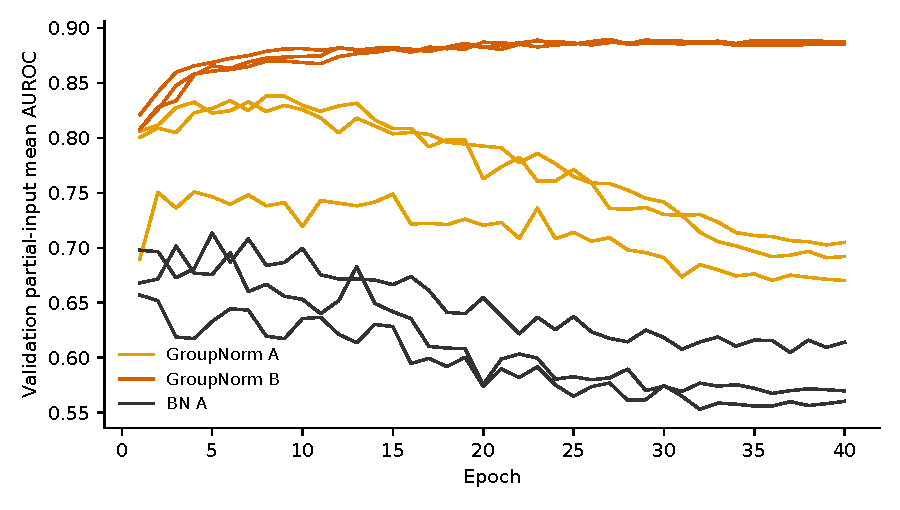
\includegraphics[width=0.7\linewidth]{figures/e8_training_dynamics.pdf}
\caption{E7: validation partial-input mean AUROC by epoch. GroupNorm A starts higher than BatchNorm A and also declines with training, which indicates reliance on the complete lead set beyond normalization statistics.}
\label{fig:e8dyn}
\end{figure}

\begin{figure}[htbp]
\centering
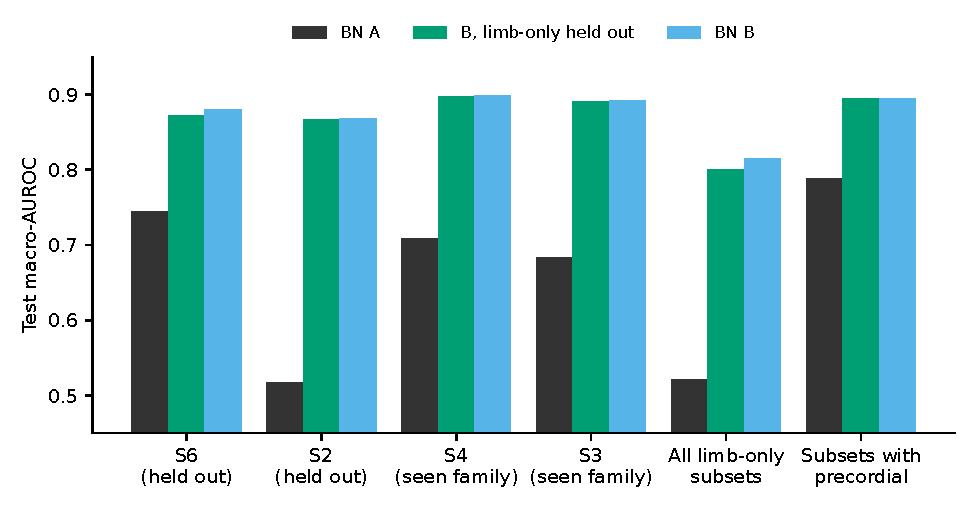
\includegraphics[width=0.8\linewidth]{figures/e9_heldout_limb_family.pdf}
\caption{E8: masked training with every limb-only partial input withheld (HO B), compared with S12-selected A and B (``BN A'' and ``BN B''). S6 and S2 are unseen in training; S4 and S3 belong to a seen family. The last two groups average over all limb-only conditions evaluated in E5 (21 conditions, 15 distinct subsets) and all other partial-input conditions (199), among the 220 partial-input conditions evaluated in E5 (4 protocol sets, 12 single-lead sets and 204 random subsets).}
\label{fig:e9}
\end{figure}

\begin{figure}[htbp]
\centering
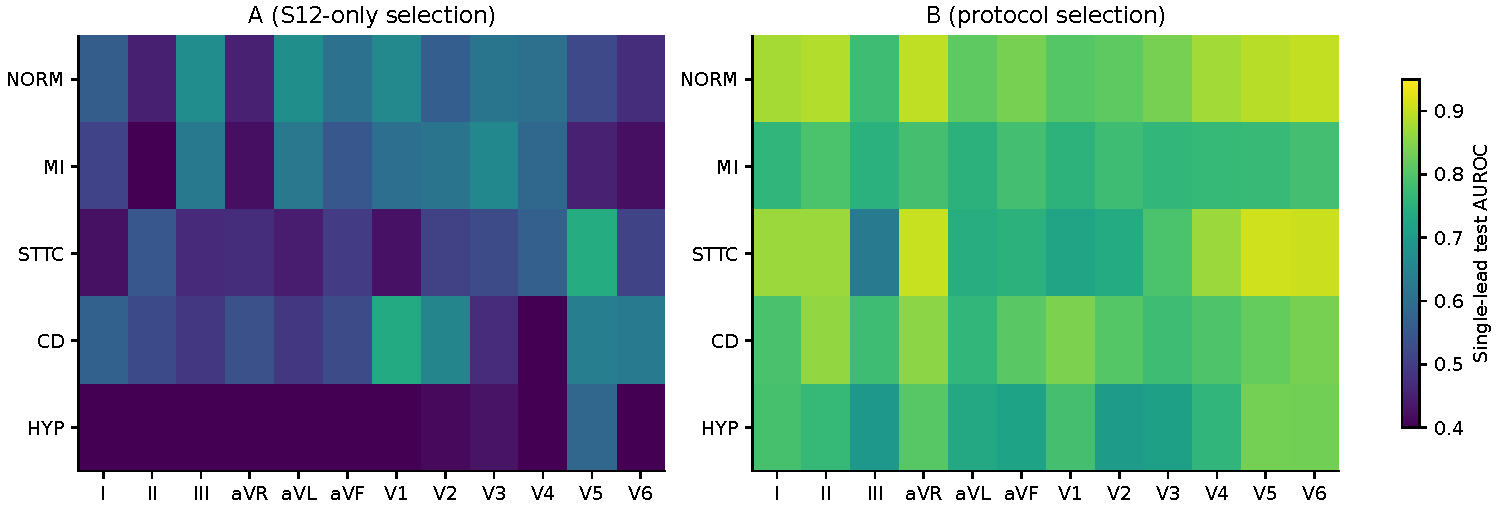
\includegraphics[width=\linewidth]{figures/e6_single_lead_per_label.pdf}
\caption{E5: per-label test AUROC with a single retained lead, for complete-input training (A, S12-only selection) and masked training (B, protocol selection).}
\label{fig:e6label}
\end{figure}

\clearpage
\section{Data audit and class examples}
\label{app:data}

The following checks cover the computational reliability of the data pipeline.
\begin{itemize}
\item \textbf{Independent reader.} On a 100-record training pilot sample, an independently implemented format-16 reader matched WFDB exactly over 1.2 million float32 values.
\item \textbf{Re-decoding.} 40 development recordings (20 + 20 sampled evenly from the training and validation splits) and 30 test recordings were re-decoded from the raw WFDB files and re-standardized with the same reader and normalization code; all values matched the stored arrays. These recomputations test consistency of the same code.
\item \textbf{Hashes and alignment.} The hashes of all original files and prepared arrays were recorded, and labels were checked against record order for every split.
\item \textbf{Normalization.} Means and variances were accumulated in float64 and stored as float32. The 0.000001\,mV floor on the standard deviation was never triggered.
\item \textbf{Test timing.} The six checkpoint hashes were fixed at 2026-10-22 18:55 UTC, and the pipeline first parsed fold-10 diagnostic codes at 20:20 UTC the same day.
\end{itemize}

\begin{figure}[htbp]
\centering
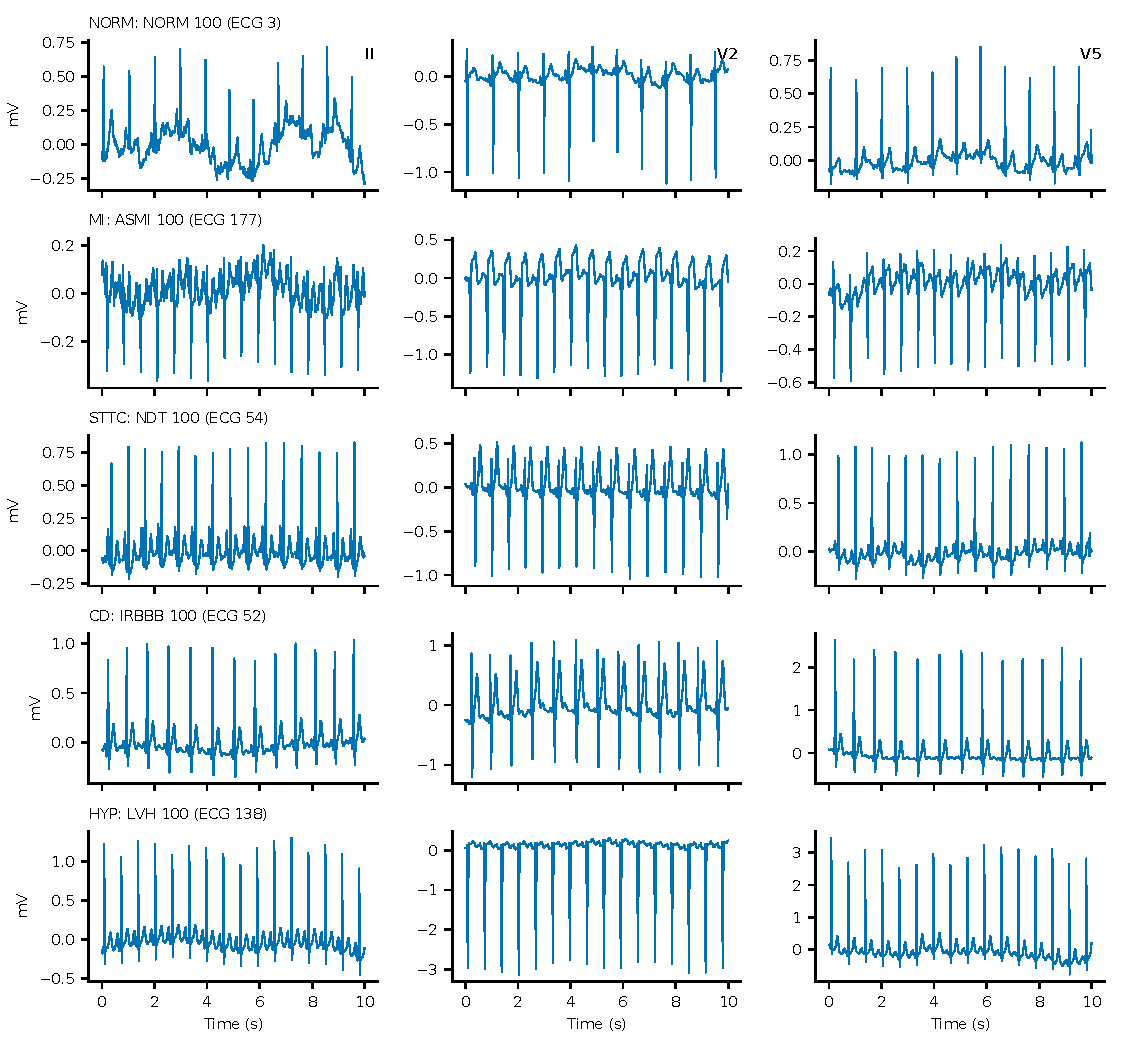
\includegraphics[width=\linewidth]{figures/appendix_class_examples.pdf}
\caption{Leads II, V2 and V5 (in mV) of one training record per diagnostic superclass. Records were selected from metadata alone: exactly one superclass, every diagnostic statement at likelihood 100, human-validated labels, age at least 18 and no PTB-XL signal-quality flag, taking the lowest ECG id per class (NORM: ECG 3; MI: ECG 177, ASMI; STTC: ECG 54, NDT; CD: ECG 52, IRBBB; HYP: ECG 138, LVH). Panel titles give the SCP codes and likelihoods. The NORM example carries no quality flag and still shows baseline wander in lead II. Anterior infarction and hypertrophy are expressed mainly in the precordial leads, so V2 and V5 are shown alongside lead II.}
\label{fig:classexamples}
\end{figure}

\clearpage
\section{Verification, implementation details and compute record}
\label{app:compute}

\begin{itemize}
\item \textbf{Test-metric verification.} An evaluation reimplemented by Codex in scikit-learn reproduced all 300 test AUROC/AP values within floating-point precision. Three bootstrap cohorts were explicitly expanded into repeated records and checked through 450 AUROC calculations; all draw-validity decisions and main percentile intervals were independently recomputed. Checkpoint hashes and model states remained unchanged.
\item \textbf{Exploratory replay.} The deterministic replay reproduced all six archived checkpoint hashes, and re-running the archived models reproduced the archived test predictions exactly (maximum absolute difference 0.0).
\item \textbf{BatchNorm re-estimation.} Each layer's running mean and variance are reset, momentum is set to none (cumulative average), and the masked records are passed forward in training mode without gradients.
\item \textbf{Random streams.} The masking sampler uses a PyTorch CPU generator (\texttt{torch.Generator}) seeded with seed plus 1,000,003. E5's random subsets draw, for each $k$, $\min(20, \binom{12}{k})$ of the $\binom{12}{k}$ combinations without replacement with a NumPy generator (seed 20261024); the full list is in the supplementary material. E9's noise and baseline wander use a \texttt{torch.Generator} seeded with $7919\times(\text{configuration index}+1)+\text{batch start}$, so every model receives identical fill values.
\item \textbf{Youden thresholds.} Candidates are all distinct validation predictions for the label; the threshold with the largest $J$ is chosen, and ties take the smallest threshold.
\item \textbf{Training cost.} The six comparison runs used 733.28 seconds of training and 185.17 seconds of repeated validation on an RTX 4060 Laptop GPU, with maximum PyTorch allocated/reserved memory 161.80/176 MiB. Dynamic loss scaling skipped 15 of 64,080 optimization attempts; training losses remained finite. Each additional model trained for E3, E4, E7, E8 and E12 took a few minutes.
\item \textbf{Rerun.} A Windows log-replacement error required one unchanged seed-43 A rerun, whose selected validation predictions reproduced exactly; the discarded attempt added 125.26/30.81 seconds of training/validation.
\item \textbf{Evaluation cost.} Test evaluation across six models and five configurations took 6.87 seconds, including startup, transfer, synchronization and metric computation; bootstrap and summarization took 21.85 seconds. The E11 subset extension took about 25 minutes of inference and 50 minutes of CPU bootstrap. These are implementation costs, not clinical-device latency.
\end{itemize}

\end{document}
